\documentclass{tufte-handout}
\usepackage{pgfplots}
\usepackage[dvipsnames]{xcolor}
\usepackage{ulem}
\usepackage{subcaption}
\usepackage{amssymb, amsmath, pgfplots, tabularx, siunitx}
\usepackage{algorithm}
\usepackage{makecell}
\usepackage{amsfonts}
\usepackage{amsthm, thmtools}
\pgfplotsset{compat = newest}

\usepackage{tikz}
\usetikzlibrary{shadings}
\usetikzlibrary{calc,arrows.meta}
\usetikzlibrary{shapes.misc}
\usetikzlibrary{positioning}
\usepackage[most]{tcolorbox}
\usepgfplotslibrary{colormaps,patchplots}

\definecolor{wp-bg}{HTML}{FDF6EF}
\definecolor{wp-text}{HTML}{2D1B0E}
\definecolor{wp-primary}{HTML}{C24A3A}
\definecolor{wp-accent}{HTML}{D4952E}
\definecolor{wp-light}{HTML}{F0DECA}
\definecolor{wp-muted}{HTML}{C4A88A}
\definecolor{wp-dark}{HTML}{1A0F07}
\definecolor{wp-code}{HTML}{FDF2E4}

\pagecolor{wp-bg}
\color{wp-text}

\hypersetup{colorlinks=true,linkcolor=wp-primary,urlcolor=wp-accent}

\let\subsubsection\subsection

% Theorem environments
\declaretheorem[style=plain, name=Defini\c{c}\~{a}o, numberwithin=section]{defn}
\declaretheorem[style=plain, name=Teorema, numberwithin=section]{thm}
\declaretheorem[style=plain, name=Lema, numberwithin=section]{lem}
\declaretheorem[style=remark, name=Exemplo, numberwithin=section]{exmp}
\declaretheorem[style=remark, name=Observa\c{c}\~{a}o, numberwithin=section]{remark}

\tikzset{basic/.style={draw,text width=1em,text badly centered}}
\tikzset{input/.style={basic,circle}}
\tikzset{weights/.style={basic,rectangle}}
\tikzset{functions/.style={basic,circle}}

\title{Friendly Introduction to Deep Generative Models\\
Image synthesis version}
\author{Vitor N. Cabral de Oliveira\\ \href{mailto:vnco@cin.ufpe.br}{vnco@cin.ufpe.br}}

\date{\today}

\begin{document}

\maketitle

\begin{abstract}
   This notebook will serve as a comprehensive repository for my notes for an introductory course about 
   eep Generative Models, with a particular focus on image generation. 
   The content will cover the following key topics:
    \begin{itemize}
    \item Style Transfer
    \item Autoencoders
    \item Variational Autoencoders
    \item Generative Adversarial Networks
    \item Diffusion Models
   \end{itemize}
   Future updates will introduce dedicated sections on energy-based models, flow-based models, and Boltzmann machines. 
   To establish a rigorous framework, a preliminary section will review the statistical learning principles that serve as the agnostic 
   mathematical foundation for generative modeling, using Hidden Markov Models as a classic introductory paradigm.
\end{abstract}

\newpage
\hypersetup{linkcolor=wp-text}
\tableofcontents
\hypersetup{linkcolor=wp-primary}
\newpage

\paragraph{Roteiro.}
Este documento percorre a evolução dos modelos generativos profundos para síntese de imagens seguindo uma progressão narrativa em que cada abordagem endereça limitações da anterior.

Começamos com \textbf{Style Transfer}, um aquecimento que demonstra como CNNs separam e recombinam conteúdo e estilo usando representações hierárquicas. Isso nos leva aos \textbf{Autoencoders}, que aprendem representações latentes compactas de forma não supervisionada. Mas autoencoders clássicos são determinísticos --- não geram novos dados. Os \textbf{VAEs} introduzem um espaço latente probabilístico que permite amostragem, porém as amostras tendem a ser borradas. As \textbf{GANs} surgem como paradigma adversarial para qualidade foto-realista, mas com treinamento instável. Os \textbf{Modelos de Difusão} oferecem qualidade similar com estabilidade, inspirando-se em processos termodinâmicos. Os \textbf{Rectified Flow Models} simplificam e aceleram a difusão aprendendo fluxos ODE diretos. Por fim, os \textbf{Modelos Baseados em Energia} oferecem uma perspectiva alternativa modelando densidades via funções de energia.

\section{Style Transfer}

\begin{defn}[Style Transfer]
A transferência de estilo é uma técnica de visão computacional que utiliza redes neurais convolucionais (CNNs) para gerar uma nova imagem que combina o conteúdo de uma imagem com o estilo artístico de outra. Essa técnica foi proposta no artigo seminal \textit{A Neural Algorithm of Artistic Style} por Leon Gatys et al. e faz uso de redes convolucionais pré-treinadas, como a ResNet50, para extrair características visuais de diferentes níveis de abstração.
\end{defn}

A metodologia se baseia na relação entre as múltiplas camadas de uma CNN, onde cada camada $l$ produz um conjunto de mapas de características $F^{l}(I)$. Esses mapas capturam informações visuais em diferentes níveis de complexidade, desde bordas e texturas nas camadas iniciais até formas e objetos nas camadas mais profundas. Assim, a CNN pode ser vista como um extrator hierárquico de características, onde cada camada contribui para a representação da imagem $I$.

O processo de transferência de estilo depende de duas imagens de entrada:
\begin{enumerate}
    \item \textbf{Imagem de conteúdo ($C$)}: Contém a estrutura e os objetos principais que serão preservados na imagem gerada.
    \item \textbf{Imagem de estilo ($S$)}: Fornece as texturas, cores e padrões artísticos que serão transferidos para a imagem final.
\end{enumerate}


A imagem gerada ($G$) é obtida por meio da otimização de uma função de perda composta, que combina a representação do conteúdo e do estilo.

\subsection{Representação do Conteúdo}

O conteúdo de uma imagem está associado às características de alto nível, como formas e objetos, que são capturados principalmente pelas camadas mais profundas da CNN. Para representar o conteúdo, utilizamos os mapas de características $F^l(C)$ e $F^l(G)$ extraídos de uma camada específica $l$ da rede.

A função de perda do conteúdo mede a diferença entre as representações da imagem de conteúdo e da imagem gerada na camada $l$. Essa diferença é calculada como o erro quadrático médio entre os mapas de características:

\begin{equation}
    \mathcal{L}_{\text{conteúdo}} (C, G, l) = \frac{1}{2} \sum_{i,j} \left(F_{ij}^l(G) - F_{ij}^l(C)\right)^2
\end{equation}

Onde:
- $F_{ij}^l(C)$ é o valor do mapa de características da imagem de conteúdo na posição $(i,j)$ da camada $l$.
- $F_{ij}^l(G)$ é o valor correspondente na imagem gerada.

\subsection{Representação do Estilo}

O estilo de uma imagem está associado às características de baixo e médio nível, como texturas, cores e padrões, que são capturados pelas correlações entre os mapas de características em \textbf{múltiplas camadas} $L$ da CNN. Para representar o estilo, utilizamos a matriz de Gram $G^l$, que mede as correlações entre os mapas de características na camada $l$.

A função de perda do estilo é definida como a soma ponderada das diferenças entre as matrizes de Gram da imagem de estilo e da imagem gerada em várias camadas:

\begin{equation}
    \mathcal{L}_{\text{estilo}} (S, G, L) = \sum_{l \in L} w_l \cdot \frac{1}{4N_l^2 M_l^2} \sum_{i,j} \left(G^l_{ij}(G) - G^l_{ij}(S)\right)^2
\end{equation}

Onde:
- $w_l$ é o peso associado à camada $l$, que controla sua contribuição para a perda total.
- $N_l$ é o número de mapas de características na camada $l$.
- $M_l$ é o tamanho espacial (altura $\times$ largura) dos mapas de características na camada $l$.
- $G^l_{ij}(S)$ e $G^l_{ij}(G)$ são os elementos das matrizes de Gram para a imagem de estilo e a imagem gerada, respectivamente.

\subsection{Otimização}

A imagem gerada $G$ é obtida minimizando uma função de perda total, que combina as perdas de conteúdo e estilo:

\begin{equation}
    \mathcal{L}_{\text{total}} (C, S, G) = \alpha \cdot \mathcal{L}_{\text{conteúdo}} (C, G, l) + \beta \cdot \mathcal{L}_{\text{estilo}} (S, G, L)
\end{equation}

Onde $\alpha$ e $\beta$ são hiperparâmetros que controlam o equilíbrio entre a preservação do conteúdo e a transferência do estilo.

Por meio de técnicas de otimização, como o gradiente descendente, a imagem gerada é iterativamente ajustada até que a perda total seja minimizada, resultando em uma imagem que combina o conteúdo de $C$ com o estilo de $S$.


O objetivo é minimizar \( \mathcal{L}_{\text{total}} \) em relação à imagem gerada \( \mathbf{G} \). Isso é feito usando Gradient Descent:
\[
\mathbf{G} \leftarrow \mathbf{G} - \eta \cdot \nabla_{\mathbf{G}} \mathcal{L}_{\text{total}}
\]
Onde \( \eta \) é a taxa de aprendizado.

\subsection{Matrizes de Gram na Transferência de Estilo}

As matrizes de Gram desempenham um papel crucial na captura do estilo de uma imagem durante o processo de transferência de estilo. Elas são usadas para medir as correlações entre os mapas de características em diferentes camadas de uma rede neural convolucional (CNN). Esta seção fornece uma explicação detalhada das matrizes de Gram, seu cálculo e sua importância na transferência de estilo.

\subsubsection{Definição das Matrizes de Gram}

Dado um conjunto de mapas de características $F^l$ extraídos de uma camada específica $l$ de uma CNN, a matriz de Gram $G^l$ é uma matriz quadrada que captura os produtos internos entre os mapas de características vetorizados. Se os mapas de características na camada $l$ têm dimensões $N_l \times M_l$ (onde $N_l$ é o número de mapas de características e $M_l$ é a dimensão espacial, ou seja, altura $\times$ largura), a matriz de Gram $G^l$ é definida como:

\[
G^l = F^l \cdot (F^l)^T
\]

Onde:
\begin{itemize}
    \item $F^l$ é a matriz de mapas de características vetorizados com dimensões $N_l \times M_l$.
    \item $(F^l)^T$ é a transposta de $F^l$.
    \item A matriz de Gram resultante $G^l$ tem dimensões $N_l \times N_l$.
\end{itemize}

Cada elemento $G^l_{ij}$ da matriz de Gram representa o produto interno entre o $i$-ésimo e o $j$-ésimo mapa de características:

\[
G^l_{ij} = \sum_{k=1}^{M_l} F^l_{ik} \cdot F^l_{jk}
\]

\subsubsection{Interpretação das Matrizes de Gram}

A matriz de Gram codifica informações sobre as correlações entre os mapas de características em uma determinada camada. Essas correlações capturam a textura e o estilo de uma imagem, pois representam a frequência com que certas características (por exemplo, bordas, cores, padrões) aparecem juntas na imagem. Por exemplo:
\begin{itemize}
    \item Valores altos na matriz de Gram indicam correlações fortes entre mapas de características específicos, o que corresponde a padrões ou texturas recorrentes na imagem.
    \item  Valores baixos indicam correlações fracas ou inexistentes, sugerindo a ausência de tais padrões.
\end{itemize}

Ao comparar as matrizes de Gram da imagem de estilo e da imagem gerada, o algoritmo de transferência de estilo garante que a imagem gerada imite a textura e o estilo da imagem de estilo.

\subsubsection{Matrizes de Gram na Função de Perda de Estilo}

A função de perda de estilo na transferência de estilo é calculada usando as matrizes de Gram da imagem de estilo ($S$) e da imagem gerada ($G$). Para uma camada específica $l$, a perda de estilo é definida como o erro quadrático médio entre as matrizes de Gram das duas imagens:

\[
\mathcal{L}_{\text{estilo}}^l (S, G) = \frac{1}{4N_l^2 M_l^2} \sum_{i,j} \left(G^l_{ij}(G) - G^l_{ij}(S)\right)^2
\]

Onde:
\begin{itemize}
    \item $G^l_{ij}(S)$ é o elemento da matriz de Gram para a imagem de estilo.
    \item $G^l_{ij}(G)$ é o elemento da matriz de Gram para a imagem gerada.
    \item $N_l$ é o número de mapas de características na camada $l$.
    \item $M_l$ é a dimensão espacial dos mapas de características na camada $l$.
\end{itemize}

A perda de estilo total é calculada como uma soma ponderada das perdas de estilo em várias camadas $L$:

\[
\mathcal{L}_{\text{estilo}} (S, G, L) = \sum_{l \in L} w_l \cdot \mathcal{L}_{\text{estilo}}^l (S, G)
\]

Onde $w_l$ é o peso atribuído à camada $l$.

\begin{exmp}[Cálculo da Matriz de Gram]

Considere um exemplo simplificado em que uma camada $l$ tem $N_l = 3$ mapas de características, cada um com dimensão espacial de $M_l = 2 \times 2 = 4$. Os mapas de características podem ser representados como:

\[
F^l = \begin{bmatrix}
1 & 2 & 3 & 4 \\
2 & 0 & 1 & 3 \\
1 & 1 & 2 & 2
\end{bmatrix}
\]

A matriz de Gram $G^l$ é calculada como:

\[
G^l = F^l \cdot (F^l)^T = \begin{bmatrix}
1 & 2 & 3 & 4 \\
2 & 0 & 1 & 3 \\
1 & 1 & 2 & 2
\end{bmatrix}
\cdot
\begin{bmatrix}
1 & 2 & 1 \\
2 & 0 & 1 \\
3 & 1 & 2 \\
4 & 3 & 2
\end{bmatrix}
= \begin{bmatrix}
30 & 20 & 20 \\
20 & 14 & 13 \\
20 & 13 & 14
\end{bmatrix}
\]

Cada elemento de $G^l$ representa a correlação entre os mapas de características correspondentes.
\end{exmp}

\subsubsection{Significância das Matrizes de Gram}

As matrizes de Gram são essenciais para a transferência de estilo porque fornecem uma maneira de quantificar e comparar a textura e o estilo das imagens. Ao minimizar a diferença entre as matrizes de Gram da imagem de estilo e da imagem gerada, o algoritmo garante que a imagem gerada adote o estilo artístico da imagem de estilo enquanto preserva o conteúdo da imagem de conteúdo.

\medskip
\noindent A separação entre conteúdo e estilo nos mostrou que redes profundas aprendem representações hierárquicas poderosas. Os Autoencoders dão o próximo passo: aprender, de forma não supervisionada, representações latentes compactas que capturam a estrutura essencial dos dados --- comprimindo sem perder o que é importante, um pré-requisito para a geração.

\section{Autoencoders}

Autoencoders (AEs) são uma técnica de aprendizado não supervisionado que visa aprender representações compactas e eficientes de dados sem a necessidade de rótulos. Eles consistem em duas redes neurais principais: o \textbf{encoder} (codificador) e o \textbf{decoder} (decodificador). O encoder transforma os dados de entrada em uma representação codificada, enquanto o decoder tenta reconstruir os dados originais a partir dessa representação. Matematicamente, um autoencoder é definido por:

\begin{equation}
    E_{\phi}: \mathcal{X} \rightarrow \mathcal{Z} \quad \text{e} \quad D_{\theta}: \mathcal{Z} \rightarrow \mathcal{X}
\end{equation}

Onde:
\begin{itemize}
    \item $E_{\phi}$ é o encoder, parametrizado por $\phi$.
    \item $D_{\theta}$ é o decoder, parametrizado por $\theta$.
    \item $\mathcal{X}$ é o espaço dos dados de entrada (por exemplo, $\mathbb{R}^m$).
    \item $\mathcal{Z}$ é o espaço latente (ou espaço codificado), geralmente de dimensão menor que $\mathcal{X}$ (por exemplo, $\mathbb{R}^n$, com $n \leq m$).
\end{itemize}

O objetivo do autoencoder é aprender uma representação compacta $z \in \mathcal{Z}$ dos dados de entrada $x \in \mathcal{X}$, de modo que a reconstrução $\hat{x} = D_{\theta}(E_{\phi}(x))$ seja o mais próxima possível de $x$.

\begin{figure*}[htbp]
\centering
\resizebox{\textwidth}{!}{%
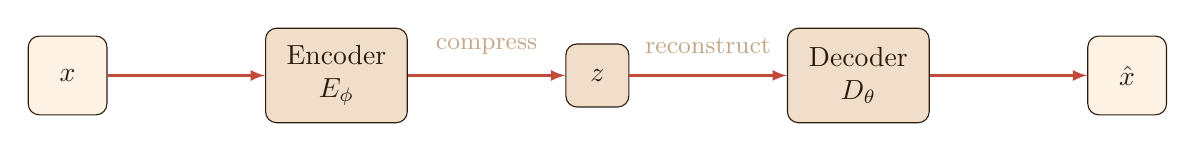
\begin{tikzpicture}[
    node distance=2.0cm, 
    auto, 
    font=\normalsize,
    >=latex
  ]
  
  % Global Style Definitions using your native wp- colors
  \tikzset{
    box/.style={draw=wp-text, fill=wp-light, rounded corners, minimum width=1.8cm, minimum height=1.2cm, text=wp-text, align=center},
    input/.style={draw=wp-text, fill=wp-code, rounded corners, minimum width=1.0cm, minimum height=1.0cm, text=wp-text, align=center},
    latent/.style={draw=wp-text, fill=wp-light, rounded corners, minimum width=0.8cm, minimum height=0.8cm, text=wp-text, align=center}
  }

  % Horizontal Pipeline
  \node (input)   [input] {$x$};
  \node (encoder) [box, right=of input] {Encoder \\ $E_\phi$};
  \node (latent)  [latent, right=of encoder] {$z$};
  \node (decoder) [box, right=of latent] {Decoder \\ $D_\theta$};
  \node (output)  [input, right=of decoder] {$\hat{x}$};

  % Connecting Edges using your primary theme color (Terracotta)
  \draw[->, wp-primary, thick] (input) -- (encoder);
  \draw[->, wp-primary, thick] (encoder) -- (latent);
  \draw[->, wp-primary, thick] (latent) -- (decoder);
  \draw[->, wp-primary, thick] (decoder) -- (output);

  % Step Metadata Labels (Muted earth tone)
  \node[above=0.15cm, wp-muted, font=\small] at ($(encoder.east)!0.5!(latent.west)$) {compress};
  \node[above=0.15cm, wp-muted, font=\small] at ($(latent.east)!0.5!(decoder.west)$) {reconstruct};

\end{tikzpicture}
}
\caption{Exemplo clássico da arquitetura de um Autoencoder (AE).}
\label{fig:ae_expanded}
\end{figure*}


\subsection{Espaço Latente}

\begin{defn}[Espaço Latente]
O espaço latente $\mathcal{Z}$ é uma representação de dimensionalidade reduzida dos dados de entrada. Para cada dado $x \in \mathcal{X}$, o encoder mapeia $x$ para um vetor 
latente $z \in \mathcal{Z}$:

\begin{equation}
    z = E_{\phi}(x)
\end{equation}

Esse vetor latente $z$ captura as características essenciais dos dados de entrada, eliminando redundâncias e ruídos.
 A dimensionalidade de $\mathcal{Z}$ é tipicamente menor que a de $\mathcal{X}$, o que permite ao autoencoder aprender uma representação compacta e eficiente.
\end{defn}

\subsection{Funcionamento do Autoencoder}

A intuição por trás de um autoencoder pode ser resumida em três etapas principais:
\begin{enumerate}
    \item \textbf{Entrada}: Um dado $x \in \mathbb{R}^D$ é fornecido como entrada.
    \item \textbf{Encoder}: O encoder mapeia $x$ para um vetor latente $z \in \mathbb{R}^d$, onde $d \ll D$:
   \begin{equation}
       z = E(x) = \sigma(W_e x + b_e)
   \end{equation}
   Aqui, $W_e$ e $b_e$ são os pesos e vieses do encoder, respectivamente, e $\sigma$ é uma função de ativação não linear (como ReLU ou sigmoide).
   \item $\mathbf{Decoder}$ O decoder reconstrói $\hat{x} \in \mathbb{R}^D$ a partir do vetor latente $z$:
   \begin{equation}
       \hat{x} = D(z) = \sigma(W_d z + b_d)
   \end{equation}
   Onde $W_d$ e $b_d$ são os pesos e vieses do decoder.
\end{enumerate}

\subsection{Função de Perda}

O objetivo do autoencoder é minimizar o erro de reconstrução, ou seja, a diferença entre a entrada original $x$ e a reconstrução $\hat{x}$. 
A função de perda mais comum é o erro quadrático médio (MSE), definido como:

\begin{equation}
    \mathcal{L}_{AE} = \mathbb{E}_{x \sim p_{\text{data}}} \left[ \Vert x - \hat{x} \Vert^2 \right]
\end{equation}

Onde:
\begin{itemize}
    \item $\mathbb{E}_{x \sim p_{\text{data}}}$ denota o valor esperado em relação à distribuição dos dados de entrada.
    \item $\Vert x - \hat{x} \Vert^2$ é a norma euclidiana ao quadrado da diferença entre $x$ e $\hat{x}$.
\end{itemize}


Ao minimizar essa função de perda, o autoencoder aprende a reconstruir os dados de entrada com a maior precisão possível, ao mesmo tempo em que compacta a informação no espaço latente.

\subsection{Variações de Autoencoders}

Além do autoencoder básico, existem várias variações que ampliam suas capacidades:
\begin{itemize}
    \item Denoising Autoencoder: Treinado para reconstruir dados a partir de entradas corrompidas por ruído.
    \item Sparse Autoencoder: Introduz uma penalidade de esparsidade no espaço latente, incentivando a ativação de apenas algumas unidades latentes.
    \item Variational Autoencoder (VAE): Modela a distribuição dos dados no espaço latente, permitindo a geração de novos dados.
    \item Convolutional Autoencoder: Utiliza camadas convolucionais no encoder e decoder, sendo especialmente útil para dados imagéticos.
\end{itemize}

\medskip
\noindent Autoencoders clássicos aprendem um mapeamento determinístico $x \rightarrow z \rightarrow \hat{x}$, excelente para compressão mas insuficiente para geração: não há estrutura probabilística que permita amostrar novos $z$ realistas. Os \textbf{Variational Autoencoders} preenchem exatamente essa lacuna, modelando o espaço latente probabilisticamente --- cada $x$ é mapeado para uma distribuição $q_\phi(z|x)$ em vez de um único vetor $z$.

\section{Variational Autoencoders (VAEs)}

Os Variational Autoencoders (VAEs) são uma extensão dos autoencoders tradicionais que incorporam conceitos de inferência probabilística. 
Enquanto autoencoders comuns aprendem uma representação determinística no espaço latente, os VAEs modelam a distribuição de probabilidade dos dados no espaço latente, permitindo a 
geração de novos dados a partir dessa distribuição. 

\begin{figure*}[htbp]
\centering
\resizebox{\textwidth}{!}{%
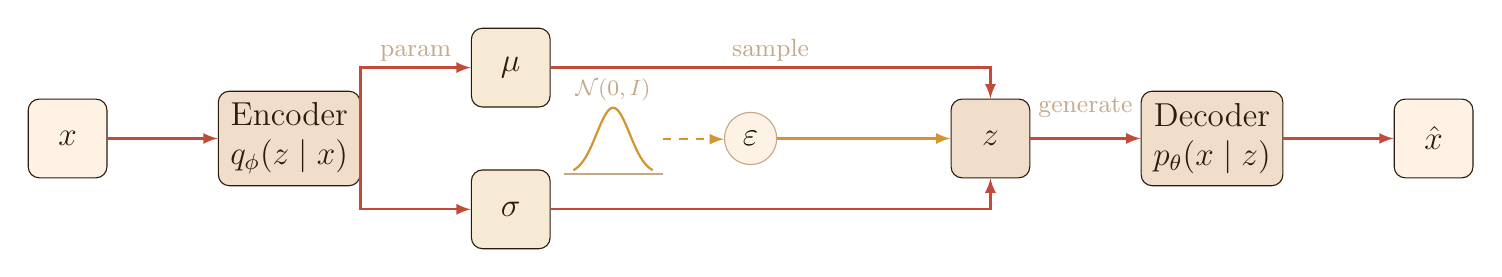
\begin{tikzpicture}[
    node distance=1.0cm and 1.4cm, 
    auto, 
    font=\large,
    >=latex
  ]
  
  % Global Style Definitions matching your exact branding
  \tikzset{
    box/.style={draw=wp-text, fill=wp-light, rounded corners, minimum width=1.8cm, minimum height=1.2cm, text=wp-text, align=center},
    input/.style={draw=wp-text, fill=wp-code, rounded corners, minimum width=1.0cm, minimum height=1.0cm, text=wp-text, align=center},
    param/.style={draw=wp-text, fill=wp-accent!20, rounded corners, minimum width=1.0cm, minimum height=1.0cm, text=wp-text, align=center},
    latent/.style={draw=wp-text, fill=wp-light, rounded corners, minimum width=1.0cm, minimum height=1.0cm, text=wp-text, align=center}
  }

  % Pipeline Nodes
  \node (input)   [input] {$x$};
  \node (encoder) [box, right=of input] {Encoder \\ $q_\phi(z \mid x)$};
  
  % Distributed Latent Parameters
  \node (mu)      [param, right=of encoder, yshift=0.9cm] {$\mu$};
  \node (sigma)   [param, right=of encoder, yshift=-0.9cm] {$\sigma$};
  
  \coordinate (gauss_center) at ($(encoder.east)!0.5!(mu.east)$);
  
  % --- EMBEDDED GAUSSIAN BELL CURVE PLOT ---
  \begin{scope}[shift={($(gauss_center)-(-2.0cm,0.9cm)$)}, scale=0.42]
    % Small axis floor
    \draw[wp-muted, thick] (-1.5,0) -- (1.5,0);
    % Plotting the normal distribution function mathematically
    \draw[domain=-1.2:1.2, samples=60, smooth, thick, wp-accent] 
      plot (\x, {2.0*exp(-\x*\x*2)});
    % Small label indicator
    \node[wp-muted, font=\footnotesize, above] at (0, 1.9) {$\mathcal{N}(0,I)$};
    
    % Âncora calibrada no fim do eixo direito (y=0) para perfeito alinhamento horizontal
    \coordinate (borda_direita_gauss) at (1.5, 1.05);
  \end{scope}

  % Reparameterization Ring (Stochastic Noise)
  \node (reparam) [draw=wp-muted, circle, fill=wp-code, inner sep=4pt, right=of mu, xshift=0.8cm, yshift=-0.9cm] {$\varepsilon$};
  
  % Target Generation Substrate
  \node (z)       [latent, right=of reparam, xshift=0.8cm] {$z$};
  \node (decoder) [box, right=of z] {Decoder \\ $p_\theta(x \mid z)$};
  \node (output)  [input, right=of decoder] {$\hat{x}$};

  % Encoder Out-routing (Orthogonal splits)
  \draw[->, wp-primary, thick] (input) -- (encoder);
  \draw[->, wp-primary, thick] (encoder.east) |- (mu.west);
  \draw[->, wp-primary, thick] (encoder.east) |- (sigma.west);

 % Força a seta a sair da borda da gaussiana e ir perfeitamente reta (0º) até a altura exata do centro de epsilon
  \draw[->, wp-accent, dashed, thick] (borda_direita_gauss) -- (reparam.west |- borda_direita_gauss);

  % Convergence paths tracking into Latent Z
  \draw[->, wp-primary, thick] (mu.east) -| (z.north);
  \draw[->, wp-primary, thick] (sigma.east) -| (z.south);
  \draw[->, wp-accent, thick] (reparam.east) -- (z.west);

  % Generation loop termination
  \draw[->, wp-primary, thick] (z) -- (decoder);
  \draw[->, wp-primary, thick] (decoder) -- (output);

  % Flawless Textual Flow Anchors (Centered mathematically in the blank channels)
  \node[above=0.4cm, wp-muted, font=\small] at ($(encoder.east)!0.5!(mu.west)$) {param};
  \node[above=0.15cm, wp-muted, font=\small] at ($(mu.east)!0.5!(z.north)$) {sample};
  \node[above=0.15cm, wp-muted, font=\small] at ($(z.east)!0.5!(decoder.west)$) {generate};

\end{tikzpicture}
}
\caption{Arquitetura de um Variational Autoencoder (VAE) detalhando o reparameterization trick em formato expandido com amostragem exógena de uma distribuição $\mathcal{N}(0, I)$.}
\label{fig:vae_expanded_final}
\end{figure*}



\subsection{Fundamentos Probabilísticos}

Ao contrário dos autoencoders tradicionais, que mapeiam diretamente uma entrada $x$ para um vetor latente $z$, os VAEs modelam a distribuição de probabilidade $p(z|x)$. No entanto, como essa distribuição é intratável, os VAEs utilizam uma abordagem variacional para aproximá-la. Especificamente, eles introduzem uma distribuição aproximada $q_{\phi}(z|x)$, parametrizada por $\phi$, que é aprendida durante o treinamento.

O objetivo do VAE é maximizar a ELBO, que é uma aproximação do logaritmo da verossimilhança dos dados. A ELBO é dada por:

\begin{equation}
    \text{ELBO} = \mathbb{E}_{q_{\phi}(z|x)} \left[ \log p_{\theta}(x|z) \right] - D_{\text{KL}}(q_{\phi}(z|x) \Vert p(z))
\end{equation}

Onde:
\begin{itemize}
\item $\mathbb{E}_{q_{\phi}(z|x)} \left[ \log p_{\theta}(x|z) \right]$ é o termo de reconstrução, que mede quão bem o decoder consegue reconstruir $x$ a partir de $z$.
\item $D_{\text{KL}}(q_{\phi}(z|x) \Vert p(z))$ é a divergência de Kullback-Leibler (KL) entre a distribuição aproximada $q_{\phi}(z|x)$ e uma distribuição pré-definida $p(z)$ (geralmente uma distribuição normal padrão $\mathcal{N}(0, I)$).
\end{itemize}

\subsection{Encoder e Decoder Probabilísticos}

No VAE, tanto o encoder quanto o decoder são modelados probabilisticamente:
\begin{enumerate}
    \item \textbf{Encoder}: O encoder mapeia a entrada $x$ para os parâmetros de uma distribuição no espaço latente, geralmente uma distribuição normal multivariada:
   \begin{equation}
       q_{\phi}(z|x) = \mathcal{N}(z; \mu_{\phi}(x), \sigma_{\phi}^2(x))
   \end{equation}
   Onde $\mu_{\phi}(x)$ e $\sigma_{\phi}^2(x)$ são a média e a variância da distribuição, respectivamente, aprendidas pelo encoder.
   \item \textbf{Decoder}: O decoder mapeia o vetor latente $z$ para os parâmetros de uma distribuição nos dados de saída. Para dados contínuos, isso geralmente é uma distribuição normal:
   \begin{equation}
       p_{\theta}(x|z) = \mathcal{N}(x; \mu_{\theta}(z), \sigma_{\theta}^2(z))
   \end{equation}
   Para dados binários, uma distribuição Bernoulli pode ser usada.

\end{enumerate} 

\subsection{Reparametrização}

Um desafio no treinamento de VAEs é a amostragem de $z$ a partir de $q_{\phi}(z|x)$, que é uma operação estocástica e não diferenciável. Para contornar esse problema, os VAEs utilizam o \textbf{truque da reparametrização}: em vez de amostrar diretamente de $q_{\phi}(z|x)$, eles amostram de uma distribuição base $\epsilon \sim \mathcal{N}(0, I)$ e transformam a amostra da seguinte forma:

\begin{equation}
    z = \mu_{\phi}(x) + \sigma_{\phi}(x) \cdot \epsilon
\end{equation}

Essa transformação torna o processo diferenciável, permitindo o uso de gradientes descendentes para otimizar os parâmetros do modelo.

\subsection{Função de Perda}

A função de perda do VAE é o negativo da ELBO, que consiste em dois termos:
\begin{enumerate}
    \item Termo de reconstrução: Mede a qualidade da reconstrução dos dados de entrada.
    \item Termo de regularização: A divergência KL, que força a distribuição aproximada $q_{\phi}(z|x)$ a se aproximar da distribuição pré-definida $p(z)$.
\end{enumerate}

Matematicamente, a função de perda é dada por:

\begin{equation}
    \mathcal{L}_{\text{VAE}} = -\mathbb{E}_{q_{\phi}(z|x)} \left[ \log p_{\theta}(x|z) \right] + D_{\text{KL}}(q_{\phi}(z|x) \Vert p(z))
\end{equation}

\subsection{Exemplo de Arquitetura}

Um VAE típico consiste em:
\begin{enumerate}
    \item Encoder: Uma rede neural que mapeia a entrada $x$ para os parâmetros $\mu_{\phi}(x)$ e $\sigma_{\phi}(x)$ da distribuição latente.
    \item Reparametrização: Amostra $z$ usando o truque da reparametrização.
    \item Decoder: Uma rede neural que mapeia $z$ para os parâmetros da distribuição de saída $p_{\theta}(x|z)$.
\end{enumerate}

\subsection{Vantagens e Desvantagens}

\paragraph{Vantagens}
\begin{itemize}
    \item Permitem a geração de novos dados a partir de uma distribuição aprendida.
    \item O espaço latente é contínuo, o que facilita a interpolação e a manipulação de dados.
    \item São baseados em fundamentos probabilísticos sólidos.
\end{itemize}


\paragraph{Desvantagens}
\begin{itemize}
    \item As amostras geradas podem ser menos nítidas ou realistas em comparação com outras técnicas, como GANs (Generative Adversarial Networks).
    \item O treinamento pode ser mais complexo devido à necessidade de otimizar a ELBO.

\end{itemize}

\medskip
\noindent VAEs oferecem um espaço latente contínuo e bem-estruturado, mas as amostras geradas tendem a ser borradas --- a perda de reconstrução penaliza desvios pixel-a-pixel, incentivando médias sobre modos plausíveis. As \textbf{Generative Adversarial Networks} introduzem um paradigma radicalmente diferente: em vez de minimizar uma distância explícita, um discriminador aprende a distinguir amostras reais de falsas, forçando o gerador a produzir amostras indistinguíveis das reais.

\section{Generative Adversarial Networks (GANs)}

As Generative Adversarial Networks (GANs) são uma classe de modelos de aprendizado profundo introduzidos por Ian Goodfellow e colaboradores em 2014. Elas são amplamente utilizadas para geração de dados, como imagens, áudio e texto. A ideia central das GANs é treinar dois modelos neurais simultaneamente: um \textbf{gerador} (generator) e um \textbf{discriminador} (discriminator), que competem entre si em um jogo de soma zero. Essa competição leva à geração de dados realistas que são indistinguíveis dos dados reais.

\begin{defn}[Jogo Minimax das GANs]
Uma GAN consiste em dois componentes principais:
\begin{enumerate}
    \item Gerador ($G$): Um modelo que gera dados a partir de um vetor de ruído aleatório $z$, geralmente amostrado de uma distribuição simples, como uma distribuição normal ou uniforme. O objetivo do gerador é produzir dados que sejam indistinguíveis dos dados reais.
    \item Discriminador ($D$): Um modelo que tenta distinguir entre dados reais (amostrados da distribuição real $p_{\text{data}}(x)$) e dados falsos (gerados pelo gerador). O discriminador é treinado para maximizar a probabilidade de classificar corretamente os dados como reais ou falsos.
\end{enumerate}

O treinamento das GANs é formulado como um jogo minimax entre o gerador e o discriminador, onde o gerador tenta enganar o discriminador, e o discriminador tenta detectar as amostras falsas. Matematicamente, o objetivo pode ser expresso como:
\end{defn}

\begin{equation}
    \min_G \max_D V(D, G) = \mathbb{E}_{x \sim p_{\text{data}}(x)} \left[ \log D(x) \right] + \mathbb{E}_{z \sim p_z(z)} \left[ \log (1 - D(G(z))) \right]
\end{equation}

Onde:
\begin{itemize}
    \item $D(x)$ é a probabilidade estimada pelo discriminador de que $x$ seja real.
    \item $G(z)$ é a amostra gerada pelo gerador a partir do vetor de ruído $z$.
    \item $p_{\text{data}}(x)$ é a distribuição dos dados reais.
    \item $p_z(z)$ é a distribuição do vetor de ruído (geralmente $\mathcal{N}(0, I)$ ou $\text{Uniform}(-1, 1)$).
\end{itemize}

\subsection{Funcionamento do Treinamento}

O treinamento de uma GAN envolve as seguintes etapas iterativas:
\begin{enumerate}
    \item Treinamento do Discriminador: Fixa-se o gerador e atualiza-se o discriminador para maximizar a função de custo $V(D, G)$. Isso envolve:
    \begin{itemize}
        \item Classificar corretamente os dados reais como reais.
        \item Classificar corretamente os dados falsos (gerados pelo gerador) como falsos.
    \end{itemize}
    \item Treinamento do Gerador: Fixa-se o discriminador e atualiza-se o gerador para minimizar a função de custo $V(D, G)$. Isso envolve:
    \begin{itemize}
        \item Gerar dados que sejam classificados como reais pelo discriminador.

    \end{itemize}
\end{enumerate}
Esse processo é repetido até que o gerador produza dados realistas e o discriminador não consiga distinguir entre dados reais e falsos.

\subsection{Funções de Perda}

A função de perda das GANs pode ser interpretada como uma medida de divergência entre a distribuição real $p_{\text{data}}(x)$ e a distribuição gerada $p_g(x)$. No entanto, o treinamento das GANs é conhecido por ser instável, o que levou ao desenvolvimento de várias variações e funções de perda alternativas, como:
\begin{itemize}
    \item GAN Padrão: Usa a função de perda binária cruzada (binary cross-entropy).
    \item Wasserstein GAN (WGAN): Utiliza a distância de Wasserstein para melhorar a estabilidade do treinamento.
    \item Least Squares GAN (LSGAN): Substitui a função de perda binária cruzada por uma função de perda quadrática.    
\end{itemize}

\subsection{Comparação com Outras Técnicas}

As GANs são frequentemente comparadas com outras técnicas de geração de dados, como Variational Autoencoders (VAEs):
\begin{itemize}
    \item GANs: Produzem amostras de alta qualidade, mas são mais difíceis de treinar e avaliar.
    \item VAEs: São mais estáveis e fornecem uma representação probabilística do espaço latente, mas as amostras geradas podem ser menos nítidas.
\end{itemize}

\subsection{Interpretação de GANs via Teoria de Jogos}

O treinamento adversarial das GANs, apresentado na Equação~4.1, pode ser formalizado como um jogo entre dois jogadores --- o gerador $G$ e o discriminador $D$. Esta subseção aprofunda essa interpretação utilizando conceitos da teoria de jogos, conforme o artigo original de Goodfellow et al. (2014).

\subsubsection{Funções de Perda Individuais}

Embora a equação minimax represente o objetivo geral do jogo, o artigo original define as funções de perda individuais do discriminador e do gerador como:

\begin{equation}
    J^{(D)}(\theta_d, \theta_g) = - \frac{1}{2} \mathbb{E}_{x \sim p_{\text{data}}(x)} \left[ \log D(x) \right] - \frac{1}{2} \mathbb{E}_{z \sim p_z(z)} \left[ \log (1 - D(G(z))) \right]
\end{equation}

\begin{equation}
    J^{(G)}(\theta_d, \theta_g) = - J^{(D)}(\theta_d, \theta_g)
\end{equation}

No entanto, para lidar com problemas de saturação e gradientes fracos no início do treinamento, o artigo original também propõe uma \textbf{alternativa} à função de perda do gerador, conhecida como \textbf{heurística de saturação não decrescente}:

\begin{equation}
    J^{(G)}(\theta_d, \theta_g) = - \frac{1}{2} \mathbb{E}_{z \sim p_z(z)} \left[ \log (D(G(z))) \right]
\end{equation}

Essa modificação fornece gradientes mais fortes para o gerador quando o discriminador rejeita facilmente as amostras geradas.

\subsubsection{Estratégias dos Jogadores}

Cada jogador (gerador e discriminador) tem uma estratégia que consiste em ajustar seus parâmetros ($\theta_g$ e $\theta_d$, respectivamente) para otimizar sua função objetivo:

\begin{enumerate}
    \item \textbf{Discriminador} ($D$): Escolhe seus parâmetros $\theta_d$ para maximizar $J^{(D)}(\theta_d, \theta_g)$. Isso envolve classificar corretamente os dados reais como reais e os dados falsos como falsos. O discriminador é atualizado usando gradiente ascendente em sua função de perda.
    \item \textbf{Gerador} ($G$): Escolhe seus parâmetros $\theta_g$ para minimizar $J^{(G)}(\theta_d, \theta_g)$, seja usando a formulação original (minimizando a divergência de Jensen-Shannon\sidenote{A divergência de Jensen-Shannon é uma derivação da divergência de Kullback-Leibler, com diferenças sutis como o resultado ser sempre um valor finito. Sua raíz quadrada é chamada de Distância de Jensen-Shannon: a similaridade das distribuição é maior quando a distância for mais próxima à zero.}) ou a heurística de saturação não decrescente. O gerador é atualizado usando algoritmos de otimização baseados em gradiente em sua função de perda.
\end{enumerate}

O treinamento das GANs pode ser visto como um processo iterativo em que os jogadores ajustam suas estratégias em resposta às ações do oponente. O artigo original sugere atualizar o discriminador $k$ vezes para cada atualização do gerador.

\begin{thm}[Equilíbrio de Nash]

Para entender o conceito de Equilíbrio de Nash em GANs, é útil defini-lo formalmente no contexto da teoria de jogos. Considere um jogo com dois jogadores, onde:

\begin{itemize}
    \item $G$ é o gerador, com espaço de estratégias $S_G$ (o conjunto de todas as possíveis distribuições que o gerador pode produzir).
    \item $D$ é o discriminador, com espaço de estratégias $S_D$ (o conjunto de todas as possíveis funções discriminadoras).
    \item $V(G, D)$ é a função de valor (ou payoff) que define o resultado do jogo para cada combinação de estratégias.
\end{itemize}

\textbf{Definição}: Um par de estratégias $(G^*, D^*)$ é um \textbf{Equilíbrio de Nash} se, e somente se, as seguintes condições forem satisfeitas:
\begin{enumerate}
    \item Melhor resposta do discriminador: Para qualquer estratégia alternativa do discriminador $D \in S_D$, temos:
    \begin{equation}
    V(G^*, D^*) \geq V(G^*, D)
    \end{equation}
    Isso significa que, dado que o gerador está jogando a estratégia $G^*$, o discriminador não pode obter um resultado melhor do que jogar $D^*$. Em outras palavras, $D^*$ é a melhor resposta do discriminador à estratégia $G^*$.
    \item Melhor resposta do gerador: Para qualquer estratégia alternativa do gerador $G \in S_G$, temos:
    \begin{equation}
    V(G^*, D^*) \leq V(G, D^*)
    \end{equation}
    Isso significa que, dado que o discriminador está jogando a estratégia $D^*$, o gerador não pode obter um resultado melhor do que jogar $G^*$. Em outras palavras, $G^*$ é a melhor resposta do gerador à estratégia $D^*$.
\end{enumerate}
    
Em termos matemáticos mais compactos:

Um par de estratégias $(G^*, D^*)$ é um Equilíbrio de Nash se:

\begin{equation}
V(G^*, D^*) = \max_{D \in S_D} V(G^*, D) = \min_{G \in S_G} V(G, D^*)
\end{equation}

No equilíbrio de Nash, nenhum jogador tem incentivo para mudar sua estratégia unilateralmente. Qualquer desvio da estratégia de equilíbrio resultará em um resultado pior para o jogador que se desviou, assumindo que o outro jogador permaneça com sua estratégia de equilíbrio.

No contexto das GANs, o equilíbrio de Nash global idealmente ocorre quando:

\begin{itemize}
    \item O gerador $G^*$ produz amostras da distribuição real de dados ($p_g(x) = p_{\text{data}}(x)$).
    \item O discriminador $D^*$ atribui uma probabilidade de $1/2$ para todas as entradas ($D^*(x) = 1/2$ para todo $x$), indicando que ele não pode distinguir entre amostras reais e geradas.
\end{itemize} 

Importante:
\begin{itemize}
    \item A existência de um equilíbrio de Nash é garantida em jogos finitos (com um número finito de jogadores e estratégias) pelo Teorema de Nash. No entanto, GANs operam em espaços de estratégias contínuos e de alta dimensão, tornando a análise mais complexa.
    \item A definição acima refere-se ao \textbf{equilíbrio de Nash puro}. Existem também \textbf{equilíbrios de Nash mistos}, onde os jogadores escolhem suas estratégias probabilisticamente.
\end{itemize}
\end{thm}

\begin{thm}[Conexão com Jensen-Shannon]

Quando o discriminador é ótimo, \textbf{minimizar a função de valor} $V(G, D)$ \textbf{é equivalente a minimizar a divergência de Jensen-Shannon (JSD)} entre $p_{\text{data}}$ e $p_g$, conforme a seguinte relação:

\begin{equation}
V(G, D^*_G) = 2 \cdot D_{JS}(p_{\text{data}} || p_g) - \log 4
\end{equation}

Isso significa que, sob condições ideais, o treinamento de GANs visa minimizar a JSD, uma medida simétrica de similaridade entre distribuições.
\end{thm}

\subsubsection{Convergência do Treinamento}

Embora o artigo original apresente uma prova teórica de convergência para um algoritmo idealizado, ele também reconhece as dificuldades práticas, como:

\begin{enumerate}
    \item \textbf{Capacidade Limitada dos Modelos}: Redes neurais têm capacidade finita.
    \item \textbf{Otimização Imperfeita}: O discriminador nem sempre atinge seu ótimo na prática.
    \item \textbf{Aproximações da Função de Perda}: A heurística de saturação não decrescente, embora útil, não possui a mesma base teórica que a minimização da JSD.
\end{enumerate}

Esses desafios levam a problemas bem conhecidos no treinamento de GANs:
\begin{itemize}
    \item \textbf{Instabilidade}: A natureza antagônica do jogo pode causar oscilações e dificultar a convergência.
    \item \textbf{Colapso de Modo}: O gerador pode aprender a produzir apenas uma variedade limitada de amostras, perdendo a diversidade da distribuição real.
\end{itemize}

\begin{exmp}[GAN Unidimensional]

Considere um caso simplificado para ilustrar o conceito de equilíbrio de Nash:
\begin{itemize}
    \item Espaço de dados unidimensional: $x \in \mathbb{R}$.
    \item Distribuição real: $p_{\text{data}}(x) = \mathcal{N}(0, 1)$ (Gaussiana padrão).
    \item Gerador: $G(z) = \theta_g z$, onde $z \sim \mathcal{N}(0, 1)$.
    \item Discriminador: $D(x) = \sigma(\theta_d x)$, onde $\sigma$ é a função sigmoide.
\end{itemize}

Neste cenário, o equilíbrio de Nash ocorre quando $\theta_g = 1$ e $\theta_d = 0$. Isso significa que:
\begin{itemize}
    \item O gerador replica perfeitamente a distribuição real.
    \item O discriminador se torna incapaz de distinguir entre dados reais e falsos, atribuindo uma probabilidade de $0,5$ para ambos.
\end{itemize}

\paragraph{Demonstração.}
Para um gerador fixo, o discriminador ótimo é:
\begin{equation}
D^*_G(x) = \frac{p_{\text{data}}(x)}{p_{\text{data}}(x) + p_g(x)} = \frac{\mathcal{N}(x; 0, 1)}{\mathcal{N}(x; 0, 1) + \mathcal{N}(x; 0, \theta_g^2)}
\end{equation}

No equilíbrio de Nash, $p_g(x) = p_{\text{data}}(x)$, o que implica $\theta_g = 1$. Nesse caso, $D^*_G(x) = 1/2$.

Para encontrar o $\theta_d$ ótimo, pode-se derivar a função de perda do discriminador em relação a $\theta_d$. Substituindo $D(x)$ pela expressão do discriminador ótimo $D^*_G(x)$ e considerando o equilíbrio de Nash ($\theta_g = 1$), onde $p_g(x) = p_{\text{data}}(x)$, a derivada se simplifica e se torna zero quando $\theta_d = 0$. Isso indica que, no equilíbrio, o discriminador se torna uma função constante, atribuindo a probabilidade de $0,5$ para qualquer entrada.

Este exemplo é extremamente simplificado e serve apenas para fins ilustrativos. Em casos reais, encontrar o equilíbrio de Nash analiticamente é inviável, e o treinamento de GANs depende de métodos numéricos para aproximá-lo.
\end{exmp}

\medskip
\noindent Apesar da qualidade impressionante das amostras, as GANs são notoriamente instáveis durante o treinamento --- colapso de modo e oscilações são desafios constantes. Os \textbf{Modelos de Difusão} oferecem uma alternativa que alcança qualidade similar, ou superior, com treinamento estável, inspirada em processos termodinâmicos de difusão e reversão.

\section{Modelos de Difusão}

Os Modelos de Difusão (Diffusion Models) são uma classe de modelos generativos que se baseiam em um processo de difusão para transformar dados reais em ruído e, em seguida, aprender a reverter esse processo para gerar novos dados. Eles têm se destacado por sua capacidade de produzir amostras de alta qualidade e por sua estabilidade de treinamento, superando desafios comuns em outras abordagens, como GANs (Generative Adversarial Networks) e VAEs (Variational Autoencoders).

\subsection{Visão Geral do Processo de Difusão}

O conceito central dos Modelos de Difusão é simular um processo de difusão, que gradualmente adiciona ruído aos dados reais até que eles se tornem indistinguíveis de ruído puro. Em seguida, o modelo aprende a reverter esse processo, transformando o ruído de volta em dados realistas. Esse processo é dividido em duas fases principais:
\begin{enumerate}
    \item \textbf{Fase de Difusão (Forward Process)}: Adiciona ruído aos dados reais em várias etapas, seguindo um esquema pré-definido.
    \item \textbf{Fase de Reversão (Reverse Process)}: Aprende a remover o ruído e reconstruir os dados originais.
\end{enumerate}

\subsection{Fase de Difusão (Forward Process)}

\begin{defn}[Processo de Difusão]
Na fase de difusão, os dados reais $\mathbf{x}_0 \sim q(\mathbf{x})$ são gradualmente corrompidos por ruído gaussiano em $T$ etapas. Em cada etapa $t$, o dado $\mathbf{x}_t$ é obtido a partir de $\mathbf{x}_{t-1}$ pela adição de ruído:

\begin{equation}
    q(\mathbf{x}_t | \mathbf{x}_{t-1}) = \mathcal{N}(\mathbf{x}_t; \sqrt{1 - \beta_t} \mathbf{x}_{t-1}, \beta_t \mathbf{I})
\end{equation}

Onde:
\begin{itemize}
    \item $\beta_t$ é um parâmetro que controla a quantidade de ruído adicionado na etapa $t$, geralmente definido por uma \textit{schedule} de variâncias.
    \item $\mathbf{x}_{t-1}$ é a amostra da etapa anterior.
    \item $\mathbf{I}$ é a matriz identidade.
\end{itemize}

Definindo $\alpha_t = 1 - \beta_t$ e $\bar{\alpha}_t = \prod_{s=1}^t \alpha_s$, podemos obter diretamente $\mathbf{x}_t$ a partir de $\mathbf{x}_0$ em uma única etapa:

\begin{equation}
    q(\mathbf{x}_t | \mathbf{x}_0) = \mathcal{N}(\mathbf{x}_t; \sqrt{\bar{\alpha}_t} \mathbf{x}_0, (1 - \bar{\alpha}_t) \mathbf{I})
\end{equation}

Isso significa que podemos amostrar $\mathbf{x}_t$ da seguinte forma:

\begin{equation}
    \mathbf{x}_t = \sqrt{\bar{\alpha}_t} \mathbf{x}_0 + \sqrt{1 - \bar{\alpha}_t} \boldsymbol{\epsilon}, \quad \text{onde } \boldsymbol{\epsilon} \sim \mathcal{N}(\mathbf{0}, \mathbf{I})
\end{equation}

No final do processo de difusão ($t = T$), o dado $\mathbf{x}_T$ é essencialmente ruído gaussiano puro, sem qualquer informação discernível sobre $\mathbf{x}_0$, dado que a \textit{schedule} de variâncias $\beta_t$ é bem definida.
\end{defn}

\subsection{Fase de Reversão (Reverse Process)}

\begin{defn}[Processo de Reversão]
A fase de reversão consiste em aprender a remover o ruído e reconstruir os dados originais. Isso é feito por meio de um modelo neural parametrizado por $\theta$ que aprende a prever a média e a variância da distribuição gaussiana que reverte o processo de difusão em cada etapa.

O processo de reversão é modelado como uma cadeia de Markov com transições gaussianas aprendidas:

\begin{equation}
    p_\theta(\mathbf{x}_{t-1} | \mathbf{x}_t) = \mathcal{N}(\mathbf{x}_{t-1}; \boldsymbol{\mu}_\theta(\mathbf{x}_t, t), \boldsymbol{\Sigma}_\theta(\mathbf{x}_t, t))
\end{equation}

Onde:
\begin{itemize}
    \item $\boldsymbol{\mu}_\theta(\mathbf{x}_t, t)$ é a média prevista pelo modelo neural.
    \item $\boldsymbol{\Sigma}_\theta(\mathbf{x}_t, t)$ é a variância prevista pelo modelo neural. Na prática, muitas vezes é fixada como $\sigma_t^2 \mathbf{I}$, onde $\sigma_t^2$ pode ser igual a $\beta_t$ ou $\frac{1 - \bar{\alpha}_{t-1}}{1 - \bar{\alpha}_t} \beta_t$.
\end{itemize}

Em vez de prever diretamente $\mathbf{x}_{t-1}$, o modelo geralmente é treinado para prever o ruído $\boldsymbol{\epsilon}$ adicionado em cada etapa. Assim, a média $\boldsymbol{\mu}_\theta$ pode ser reparametrizada como:

\begin{equation}
    \boldsymbol{\mu}_\theta(\mathbf{x}_t, t) = \frac{1}{\sqrt{\alpha_t}} \left( \mathbf{x}_t - \frac{\beta_t}{\sqrt{1 - \bar{\alpha}_t}} \boldsymbol{\epsilon}_\theta(\mathbf{x}_t, t) \right)
\end{equation}

Portanto, o processo de amostragem para gerar $\mathbf{x}_{t-1}$ a partir de $\mathbf{x}_t$ é:

\begin{equation}
    \mathbf{x}_{t-1} = \frac{1}{\sqrt{\alpha_t}} \left( \mathbf{x}_t - \frac{\beta_t}{\sqrt{1 - \bar{\alpha}_t}} \boldsymbol{\epsilon}_\theta(\mathbf{x}_t, t) \right) + \sigma_t \mathbf{z}, \quad \text{onde } \mathbf{z} \sim \mathcal{N}(\mathbf{0}, \mathbf{I})
\end{equation}
\end{defn}

\subsection{Função de Perda}

O treinamento dos Modelos de Difusão é baseado na maximização da verossimilhança dos dados de treinamento. No entanto, a verossimilhança exata é intratável. Em vez disso, os modelos de difusão são treinados otimizando um limite inferior variacional (ELBO) na log-verossimilhança negativa.

Uma simplificação comum da função de perda é:

\begin{equation}
    \mathcal{L}(\theta) = \mathbb{E}_{t, \mathbf{x}_0, \boldsymbol{\epsilon}} \left[ \left\| \boldsymbol{\epsilon} - \boldsymbol{\epsilon}_\theta(\sqrt{\bar{\alpha}_t} \mathbf{x}_0 + \sqrt{1 - \bar{\alpha}_t} \boldsymbol{\epsilon}, t) \right\|^2 \right]
\end{equation}

Onde:
\begin{itemize}
    \item $t$ é a etapa de difusão, amostrada uniformemente entre $1$ e $T$.
    \item $\mathbf{x}_0$ é o dado real.
    \item $\boldsymbol{\epsilon} \sim \mathcal{N}(\mathbf{0}, \mathbf{I})$ é o ruído adicionado durante a fase de difusão.
    \item $\boldsymbol{\epsilon}_\theta(\mathbf{x}_t, t)$ é o ruído previsto pelo modelo, onde $\mathbf{x}_t = \sqrt{\bar{\alpha}_t} \mathbf{x}_0 + \sqrt{1 - \bar{\alpha}_t} \boldsymbol{\epsilon}$.
\end{itemize}

Essa função de perda simplesmente compara o ruído real adicionado durante o processo de difusão com o ruído previsto pelo modelo.

\subsection{Vantagens dos Modelos de Difusão}

Os Modelos de Difusão apresentam várias vantagens em relação a outras técnicas generativas:
\begin{itemize}
    \item \textbf{Estabilidade de Treinamento}: Ao contrário das GANs, que podem sofrer com instabilidade e colapso de moda, os Modelos de Difusão são mais estáveis e previsíveis.
    \item \textbf{Qualidade das Amostras}: Eles são capazes de gerar amostras de alta qualidade, especialmente em tarefas como geração de imagens.
    \item \textbf{Flexibilidade}: Podem ser aplicados a diferentes tipos de dados, como imagens, áudio e vídeos.
    \item \textbf{Fundamentação Teórica}: Baseiam-se em um processo bem definido de difusão e reversão, o que facilita a análise e a interpretação.
\end{itemize}

\subsection{Comparação com Outras Técnicas}

Em comparação com outras abordagens generativas, como GANs e VAEs, os Modelos de Difusão oferecem:
\begin{itemize}
    \item \textbf{Melhor Qualidade}: As amostras geradas tendem a ser mais nítidas e realistas.
    \item \textbf{Maior Estabilidade}: O treinamento é menos propenso a problemas como colapso de moda.
    \item \textbf{Custo Computacional}: O treinamento e a geração podem ser mais lentos devido ao grande número de etapas de difusão e reversão.
\end{itemize}

\subsection{Exemplo de Arquitetura: DDPM e U-Net}

Um exemplo popular de arquitetura para Modelos de Difusão é o Denoising Diffusion Probabilistic Models (DDPM), que utiliza uma rede neural U-Net para prever o ruído $\boldsymbol{\epsilon}_\theta(\mathbf{x}_t, t)$ em cada etapa de reversão. A U-Net é eficaz para capturar informações em múltiplas escalas, o que é crucial para a qualidade das amostras geradas.

A arquitetura U-Net consiste em um caminho de contração (encoder) que captura o contexto e um caminho de expansão (decoder) que permite a localização precisa. A U-Net também possui conexões residuais entre o encoder e o decoder, o que ajuda a preservar os detalhes finos durante o processo de geração.

\subsection{Stable Diffusion}

O Stable Diffusion é uma variação dos Modelos de Difusão que opera no \textbf{espaço latente} de um autoencoder variacional (VAE) pré-treinado, em vez de operar diretamente no espaço de pixels. Isso traz algumas vantagens:

\begin{enumerate}
    \item \textbf{Eficiência Computacional}: Trabalhar em um espaço latente de menor dimensão reduz significativamente o custo computacional do processo de difusão e reversão.
    \item \textbf{Velocidade de Amostragem}: A geração de amostras se torna mais rápida, pois o processo de reversão ocorre em um espaço de menor dimensão.
    \item \textbf{Qualidade Aprimorada}: O modelo pode se concentrar em capturar a semântica e a estrutura de alto nível dos dados, enquanto o VAE cuida dos detalhes de baixo nível.
\end{enumerate}

\subsubsection{Funcionamento do Stable Diffusion}

\begin{enumerate}
    \item \textbf{Treinamento do VAE}: Um VAE é treinado para comprimir imagens em um espaço latente de menor dimensão. O encoder do VAE mapeia uma imagem $\mathbf{x}$ para uma representação latente $\mathbf{z} = E(\mathbf{x})$, e o decoder reconstrói a imagem a partir da representação latente: $\mathbf{x} \approx D(\mathbf{z})$.
    \item \textbf{Difusão no Espaço Latente}: O processo de difusão é aplicado às representações latentes $\mathbf{z}$ em vez das imagens originais $\mathbf{x}$. Isso significa que $\mathbf{z}_t$ é obtido a partir de $\mathbf{z}_0$ (que é a representação latente de $\mathbf{x}_0$) adicionando ruído de acordo com a \textit{schedule} de variâncias.
    \item \textbf{Modelo de Difusão Condicionado}: Um modelo de difusão, geralmente uma U-Net, é treinado para reverter o processo de difusão no espaço latente. Esse modelo pode ser condicionado a informações adicionais, como texto (para geração de imagem a partir de texto) ou máscaras de segmentação (para edição de imagens).
    \item \textbf{Geração de Amostras}: Para gerar uma nova amostra, o processo de reversão é executado no espaço latente, começando com ruído gaussiano puro $\mathbf{z}_T$. Em seguida, o decoder do VAE é usado para mapear a representação latente gerada $\mathbf{z}_0$ de volta para o espaço de pixels, produzindo a imagem final $\mathbf{x} = D(\mathbf{z}_0)$.
\end{enumerate}

\subsubsection{Arquitetura do Stable Diffusion}

O Stable Diffusion geralmente usa uma arquitetura U-Net para o modelo de difusão no espaço latente. Além disso, ele pode incorporar mecanismos de atenção cruzada (cross-attention) para condicionar a geração a entradas de texto. Isso permite que o modelo gere imagens que correspondam a descrições textuais específicas.

\textbf{Em resumo}, o Stable Diffusion é uma abordagem eficiente e poderosa para a geração de imagens de alta qualidade, combinando a força dos Modelos de Difusão com a eficiência de trabalhar em um espaço latente aprendido por um VAE.
\medskip
\noindent Modelos de Difusão produzem resultados excelentes, mas seu processo de amostragem é lento --- são necessárias centenas ou milhares de etapas para gerar uma única imagem. Os \textbf{Modelos Baseados em Fluxo} oferecem alternativas que repensam fundamentalmente como conectar ruído e dados. Dentro dessa família, duas abordagens se destacam: os \textbf{Normalizing Flows}, que constroem transformações invertíveis e estáticas entre distribuições, e os \textbf{Rectified Flow Models}, que aprendem fluxos ODE dinâmicos para conectar ruído a dados de forma mais direta.

\section{Modelos Baseados em Fluxo (Flow-based Models)}

Suponha que queremos gerar imagens de rostos. Poderíamos começar com ruído puro --- uma distribuição Gaussiana em centenas de dimensões --- e gradualmente transformá-lo em algo que se pareça com um rosto. A questão central dos modelos baseados em fluxo é: \textbf{como construir uma transformação que seja simultaneamente expressiva o suficiente para gerar dados complexos e tratável o suficiente para que possamos calcular probabilidades exatas?}

Diferentemente de VAEs (que maximizam um limite inferior, a ELBO) e GANs (que não modelam densidade alguma), muitos modelos baseados em fluxo permitem o \textbf{cálculo exato da verossimilhança} dos dados --- uma propriedade fundamental para comparação objetiva entre modelos e para aplicações que exigem densidades precisas, como compressão e detecção de anomalias.

\subsection{Intuição: Como uma Transformação Altera a Densidade}

Para entender a matemática dos Normalizing Flows, comece com um exemplo unidimensional simples. Considere $Z \sim \mathcal{N}(0, 1)$ e uma transformação linear $X = f(Z) = 3Z + 1$. Como a densidade de $Z$ se transforma na densidade de $X$? A resposta é a \textbf{fórmula de mudança de variáveis}:

\begin{equation}
p_X(x) = p_Z(f^{-1}(x)) \cdot \left| \frac{d}{dx} f^{-1}(x) \right|
         = p_Z\!\left(\frac{x-1}{3}\right) \cdot \frac{1}{3}
\end{equation}

O termo $1/3$ é o \textbf{fator de distorção de volume}: a transformação linear esticou o eixo por um fator de 3, então a densidade precisa ser comprimida por $1/3$ para que a probabilidade total continue integrando a 1. Esse fator é, em 1D, o valor absoluto da derivada --- o análogo unidimensional do determinante Jacobiano.

\subsubsection{Por que o Determinante Jacobiano Representa Distorção de Volume}

Em $d$ dimensões, o Jacobiano $J_f(x)$ é a matriz $d \times d$ das derivadas parciais de $f$ no ponto $x$. O determinante $|\det J_f(x)|$ mede quanto a transformação $f$ estica (ou comprime) o volume de uma região infinitesimal ao redor de $x$:

\begin{itemize}
    \item $|\det J| = 1$: volume preservado (a área não muda --- como uma rotação pura).
    \item $|\det J| > 1$: volume expandido (a densidade diminui naquela região).
    \item $|\det J| < 1$: volume contraído (a densidade aumenta naquela região).
\end{itemize}

\begin{thm}[Mudan\c{c}a de Vari\'{a}veis]
Seja $f_\theta: \mathbb{R}^d \rightarrow \mathbb{R}^d$ uma função invertível e diferenciável que mapeia um dado $x$ a uma representação latente $z = f_\theta(x)$. A densidade de $x$ é:

\begin{equation}
p_X(x) = p_Z(f_\theta(x)) \cdot \left| \det J_{f_\theta}(x) \right|
\end{equation}

Em escala logarítmica (mais estável numericamente):

\begin{equation}
\log p_X(x) = \log p_Z(f_\theta(x)) + \log \left| \det J_{f_\theta}(x) \right|
\end{equation}
\end{thm}

O treinamento de um Normalizing Flow maximiza essa log-verossimilhança exata sobre os dados de treinamento: $\mathcal{L}(\theta) = -\mathbb{E}_{x \sim p_{\text{data}}}[\log p_X(x)]$. Isso contrasta diretamente com VAEs, que maximizam um limite inferior (ELBO), e com GANs, que não modelam verossimilhança alguma.

\subsection{Normalizing Flows}

\begin{defn}[Normalizing Flow]
Um Normalizing Flow é um difeomorfismo $f_\theta: \mathbb{R}^d \rightarrow \mathbb{R}^d$ --- uma transformação invertível e diferenciável --- que mapeia a distribuição dos dados $p_{\text{data}}(x)$ a uma distribuição latente simples $p_Z(z)$, tipicamente $\mathcal{N}(0, I)$. Amostrar do modelo é simples: $x = f_\theta^{-1}(z)$ com $z \sim p_Z$.
\end{defn}

O nome ``flow'' (fluxo) vem da composição de $K$ transformações: $f_\theta = f_1 \circ f_2 \circ \cdots \circ f_K$. Cada $f_k$ deve ser invertível e ter Jacobiano computável. A composição ``flui'' a distribuição simples através de deformações sucessivas até atingir a distribuição alvo.

\subsubsection{O Desafio do Determinante Jacobiano}

A fórmula de mudança de variáveis esconde um problema computacional: para uma matriz $d \times d$ genérica, $\det J$ requer $O(d^3)$ operações. Para uma imagem de $64 \times 64$ pixels em RGB, $d = 12288$, e $O(d^3) \approx 10^{12}$ --- completamente inviável. Precisamos de uma arquitetura em que o cálculo do determinante seja eficiente.

\subsection{Affine Coupling Layers}

A solução canônica para o problema do Jacobiano são as \textbf{affine coupling layers}, introduzidas no NICE (Dinh et al., 2014) e popularizadas pelo RealNVP (Dinh et al., 2016).

\begin{defn}[Affine Coupling Layer]
Uma coupling layer divide a entrada em duas partes $x = [x_a, x_b]$ e aplica:

\begin{align}
z_a &= x_a \\
z_b &= s_\theta(x_a) \cdot x_b + t_\theta(x_a)
\end{align}

Onde $s_\theta$ (scale) e $t_\theta$ (translate) são redes neurais arbitrárias que atuam apenas sobre $x_a$. A inversa é imediata:

\begin{align}
x_a &= z_a \\
x_b &= (z_b - t_\theta(z_a)) / s_\theta(z_a)
\end{align}
\end{defn}

\subsubsection{Por que o Determinante é Triangul\={a}r}

A chave da eficiência está na estrutura do Jacobiano. Como $z_a = x_a$, a derivada $\partial z_a / \partial x_a = I$ (identidade) e $\partial z_a / \partial x_b = 0$. Como $z_b$ depende de $x_a$ (através de $s_\theta$ e $t_\theta$) mas não de $x_b$, temos $\partial z_b / \partial x_b = \text{diag}(s_\theta(x_a))$. A matriz resultante é triangular inferior por blocos:

\begin{equation}
J = \begin{pmatrix}
I & 0 \\
\partial z_b / \partial x_a & \text{diag}(s_\theta(x_a))
\end{pmatrix}
\end{equation}

O determinante é o produto dos elementos da diagonal: $\det J = \prod_i s_\theta(x_a)_i$, computável em $O(d)$ independentemente da complexidade de $s_\theta$ e $t_\theta$. Isso torna o treinamento viável mesmo para espaços de alta dimensão.

\begin{exmp}[Coupling Layer Simples]
Considere uma coupling layer com entrada $x = [3, 7]$, dividida como $x_a = [3]$, $x_b = [7]$. Suponha que as redes retornem $s_\theta(3) = 2$ e $t_\theta(3) = 1$. A saída é:

\begin{align}
z_a &= x_a = 3 \\
z_b &= 2 \cdot 7 + 1 = 15
\end{align}

A inversa recupera $x_b = (15 - 1) / 2 = 7$. O determinante Jacobiano é $\det J = 2$, indicando que a transformação esticou o eixo $x_b$ por um fator de 2 --- a densidade na direção $x_b$ é reduzida pela metade.
\end{exmp}

\subsection{Empilhando Camadas: NICE, RealNVP e Glow}

Uma única coupling layer tem capacidade limitada --- metade das dimensões passa inalterada. A solução é \textbf{empilhar} múltiplas camadas, alternando a cada passo quais dimensões são transformadas e quais passam diretamente:

\begin{itemize}
    \item \textbf{NICE} (2014): Usa coupling layers \textit{aditivas} ($s_\theta = 1$, apenas $t_\theta$). O determinante é sempre 1 (volume preservado). Simples, mas limitado em expressividade.
    \item \textbf{RealNVP} (2016): Introduz o fator de escala $s_\theta$, permitindo compressão e expansão de volume. Alterna a divisão das dimensões a cada camada usando padrões de máscara (checkerboard, channel-wise).
    \item \textbf{Glow} (2018): Substitui as permutações fixas por convoluções $1 \times 1$ \textit{invertíveis}, que aprendem a misturar canais de forma otimizada. Introduz também \texttt{actnorm} (normalização por ativação) para estabilizar o treinamento.
\end{itemize}

O empilhamento de $K$ camadas produz $f_\theta = f_1 \circ \cdots \circ f_K$, cujo log-determinante é a soma dos log-determinantes individuais:

\begin{equation}
\log \det J_{f_\theta}(x) = \sum_{k=1}^K \log \det J_{f_k}(x_k)
\end{equation}

\subsection{Vantagens e Limitações}

\begin{itemize}
    \item \textbf{Log-verossimilhança exata}: Diferentemente de VAEs (ELBO) e GANs (sem verossimilhança), Normalizing Flows fornecem a densidade exata dos dados, permitindo comparação objetiva entre modelos.
    \item \textbf{Amostragem e inferência bidirecionais}: A invertibilidade permite tanto gerar ($z \rightarrow x$) quanto codificar ($x \rightarrow z$), útil para compressão, interpolação e detecção de anomalias (amostras com baixa verossimilhança são anomalias).
    \item \textbf{Representação latente interpretável}: Manipulações no espaço $z$ (interpolação linear, operações aritméticas) produzem mudanças semanticamente significativas no espaço $x$.
    \item \textbf{Limitação arquitetural}: A invertibilidade exige que a dimensionalidade seja preservada em cada camada --- a arquitetura é severamente restrita comparada a modelos não-invertíveis.
    \item \textbf{Custo computacional}: Cada coupling layer requer duas passagens pela rede (forward + inverse em treinamento), e o empilhamento de dezenas de camadas torna o treinamento caro.
    \item \textbf{Escalabilidade limitada}: Modelos como Glow exigem GPUs de alta memória e não escalam para megapixels tão bem quanto modelos de difusão.
\end{itemize}

\medskip
\noindent Enquanto Normalizing Flows constroem uma transformação estática e invertível, os Rectified Flow Models adotam uma abordagem dinâmica: aprendem um campo vetorial que define uma ODE conectando ruído a dados. A diferença fundamental é que Normalizing Flows mapeiam cada ponto a um único ponto correspondente (bijection), enquanto Rectified Flows definem uma trajetória contínua no tempo.

\subsection{Rectified Flow Models}

Os Rectified Flow Models (Liu et al., 2022) surgem como uma evolução direta dos Modelos de Difusão, endereçando sua principal limitação prática: o grande número de etapas necessário para amostragem. Enquanto modelos como DDPM tipicamente requerem centenas ou milhares de passos de denoising --- cada um exigindo uma avaliação da rede neural --- os Rectified Flows aprendem um fluxo ODE determinístico que conecta ruído a dados de forma mais direta.

\subsubsection{Por que a Difusão é Lenta?}

Em um modelo de difusão, o processo reverso segue uma cadeia estocástica que gradualmente remove ruído ao longo de $T$ passos. A cada passo, o modelo prevê o ruído residual e subtrai uma fração. Essa trajetória é inerentemente tortuosa: o caminho percorrido no espaço de dados é muito mais longo que a distância geométrica entre o ruído e o dado.

A ideia central dos Rectified Flows é \textbf{retificar} (endireitar) esse caminho, aprendendo um fluxo determinístico cujas trajetórias são tão retas quanto possível.

\subsubsection{Fundamentos Matemáticos}

Seja $x_0 \sim p_{\text{data}}(x)$ uma amostra real e $x_1 \sim \mathcal{N}(0, I)$ uma amostra de ruído. Um Rectified Flow modela um campo vetorial $v: \mathbb{R}^d \times [0, 1] \rightarrow \mathbb{R}^d$ que define uma ODE:

\begin{equation}
\frac{dx_t}{dt} = v(x_t, t), \quad t \in [0, 1]
\end{equation}

Partindo de $x_1$ em $t=1$ e integrando a ODE reversamente, obtemos $x_0$ em $t=0$. A trajetória $x_t$ é uma interpolação linear entre ruído e dado:

\begin{equation}
x_t = (1 - t) x_0 + t x_1
\end{equation}

O campo vetorial ideal deve apontar de $x_1$ para $x_0$, ou seja, $v(x_t, t) = x_0 - x_1$ em cada ponto da trajetória. O modelo aprende a prever exatamente essa direção.

\subsubsection{Função de Perda (Flow Matching)}

O treinamento minimiza uma perda de correspondência de fluxo (flow matching):

\begin{equation}
\mathcal{L}_{\text{RF}}(\theta) = \mathbb{E}_{t \sim \mathcal{U}[0,1], \, x_0 \sim p_{\text{data}}, \, x_1 \sim \mathcal{N}(0,I)} \left[ \left\| v_\theta(x_t, t) - (x_0 - x_1) \right\|^2 \right]
\end{equation}

Onde $x_t = (1 - t) x_0 + t x_1$. O modelo aprende a prever a direção $x_0 - x_1$ em cada ponto da trajetória. Note a semelhança com a perda de denoising dos modelos de difusão: enquanto o DDPM prevê o ruído $\boldsymbol{\epsilon}$ adicionado, o Rectified Flow prevê a diferença entre dado e ruído. Ambos são equivalentes em espírito, mas o flow matching permite trajetórias mais curtas.

\subsubsection{Processo de Retificação (Reflow)}

Uma propriedade única dos Rectified Flows é a \textbf{retificação iterativa}. Após treinar um campo $v_\theta$ inicial, as trajetórias geradas podem ainda ser curvas. O processo de \textit{reflow} as endireita progressivamente:

\begin{enumerate}
    \item Amostramos pares $(x_0, x_1)$ da distribuição conjunta induzida pelo fluxo atual (simulamos a ODE e registramos os pontos inicial e final).
    \item Treinamos um novo campo $v'_\theta$ usando esses pares como supervisão direta.
    \item Repetimos até que as trajetórias se tornem linhas retas.
\end{enumerate}

Cada iteração de reflow reduz a curvatura das trajetórias. O processo converge para um fluxo cujas trajetórias são tão retas quanto possível, permitindo amostragem em pouquíssimas etapas --- até uma única etapa. Essa é a razão pela qual modelos como Stable Diffusion 3 e SDXL Turbo conseguem gerar imagens de alta qualidade em 1--4 passos.

\subsubsection{Vantagens e Aplicações}

\begin{itemize}
    \item \textbf{Amostragem rápida}: 1--50 passos vs.~1000 do DDPM tradicional. Um passo já produz amostras reconhecíveis; 4--8 passos são suficientes para qualidade comparável a diffusion com 50 passos.
    \item \textbf{Simplicidade}: A perda de flow matching é mais simples que a ELBO dos modelos de difusão --- não requer \textit{reweighting terms} ou schedules complexas de ruído. Basta prever $x_0 - x_1$.
    \item \textbf{Determinismo}: A ODE define um mapeamento determinístico entre ruído e dados, permitindo interpolações consistentes (transições suaves entre imagens) e edição controlada.
    \item \textbf{Estado-da-arte}: O Stable Diffusion 3 utiliza Rectified Flow como mecanismo de geração principal, e o fluxo retificado é o paradigma dominante em modelos de código aberto modernos.
\end{itemize}

\subsection{Comparação entre os Paradigmas}

\medskip
\noindent
\begin{tabularx}{\textwidth}{l X X X}
\hline
\textbf{Propriedade} & \textbf{Normalizing Flow} & \textbf{Rectified Flow} & \textbf{Diffusion} \\
\hline
Invertibilidade & Sim (por construção) & Não & Não \\
NLL exata & Sim & Não (ELBO aproximado) & Não (ELBO) \\
Passos de amostragem & 1 & 1--50 & 10--1000 \\
Estabilidade de treino & Alta & Alta & Alta \\
Flexibilidade arquitetural & Baixa (invertível) & Alta (qualquer arquitetura) & Alta (qualquer arquitetura) \\
\hline
\end{tabularx}

\medskip
\noindent Enquanto Diffusion e Flow-based models transformam ruído em dados através de processos sequenciais, os \textbf{Modelos Baseados em Energia} oferecem uma perspectiva fundamentalmente diferente: em vez de aprender um processo de transformação, eles modelam diretamente uma \textit{paisagem de energia} que atribui valores baixos a amostras plausíveis e valores altos a amostras irreais. A geração de dados se torna então um problema de encontrar os vales nessa paisagem.

\section{Modelos Baseados em Energia}

Os Modelos Baseados em Energia (Energy-Based Models, EBMs) oferecem uma perspectiva fundamentalmente diferente para modelagem generativa. Em vez de modelar explicitamente uma distribuição de probabilidade (VAEs), treinar um gerador adversarial (GANs) ou modelar um processo de difusão, os EBMs aprendem uma \textbf{função de energia} $E_\theta(x): \mathbb{R}^d \rightarrow \mathbb{R}$ que atribui valores escalares a cada ponto do espaço de dados.

A intuição vem da física: sistemas físicos tendem naturalmente a estados de menor energia. Uma bola em um relevo irregular rola para os vales; analogamente, uma amostra no espaço de dados deve ``rolar'' para regiões de baixa energia, que correspondem a padrões plausíveis (rostos, objetos, texturas). Regiões de alta energia correspondem a ruído ou configurações irreais.

\subsection{Intuição: A Paisagem de Energia}

Imagine um conjunto de dígitos manuscritos MNIST. Cada imagem $28 \times 28$ é um ponto em um espaço de 784 dimensões. A maioria desses pontos --- escolhidos aleatoriamente --- parece ruído. Apenas uma fração minúscula do espaço corresponde a dígitos reais. Um EBM aprende uma função $E_\theta(x)$ que atribui:

\begin{itemize}
    \item \textbf{Energia baixa} ($E_\theta(x) \ll 0$): para imagens que se parecem com dígitos reais (vales na paisagem).
    \item \textbf{Energia alta} ($E_\theta(x) \gg 0$): para ruído ou imagens irreais (picos na paisagem).
\end{itemize}

Para \textbf{gerar} uma nova amostra, partimos de um ponto qualquer no espaço e seguimos o gradiente descendente da energia até encontrar um vale. Para \textbf{classificar}, comparamos as energias atribuídas por diferentes modelos treinados para cada classe. Para \textbf{detectar anomalias}, medimos a energia de uma nova amostra: se for alta, provavelmente está fora da distribuição de treinamento.

\subsection{Formulação Matemática}

A conexão entre energia e probabilidade é dada pela \textbf{distribuição de Boltzmann} (ou Gibbs):

\begin{thm}[Distribuição de Boltzmann]
Um Energy-Based Model define uma distribuição de probabilidade sobre o espaço de dados $x \in \mathbb{R}^d$ através de uma função de energia $E_\theta(x)$:

\begin{equation}
p_\theta(x) = \frac{\exp(-E_\theta(x))}{Z_\theta}, \qquad
Z_\theta = \int \exp(-E_\theta(x)) \, dx
\end{equation}
\end{thm}

Onde:
\begin{itemize}
    \item $E_\theta(x): \mathbb{R}^d \rightarrow \mathbb{R}$ é a função de energia, parametrizada por $\theta$ (tipicamente uma rede neural). Quanto menor a energia, maior a probabilidade.
    \item $Z_\theta$ é a \textbf{constante de normalização} (ou função de partição), que assegura que $\int p_\theta(x) \, dx = 1$.
\end{itemize}

\subsubsection{O Problema Central: $Z_\theta$ é Intratável}

O desafio fundamental dos EBMs é que $Z_\theta$ é computacionalmente intratável: requer integração sobre todo o espaço de dados. Para imagens $64 \times 64$ RGB, isso significa integrar sobre $64 \times 64 \times 3 = 12288$ dimensões. Mesmo métodos numéricos aproximados falham nessa escala.

Isso contrasta diretamente com outros modelos:
\begin{itemize}
    \item \textbf{Normalizing Flows}: calculam $p(x)$ exatamente via mudança de variáveis.
    \item \textbf{Modelos Autoregressivos}: fatoram $p(x) = \prod p(x_i | x_{<i})$, eliminando a necessidade de $Z$.
    \item \textbf{VAEs e Diffusion}: maximizam um limite inferior (ELBO), evitando $Z$.
\end{itemize}
Os EBMs precisam de métodos especiais de treinamento que contornem a intratabilidade de $Z$.

\subsection{Treinamento: Como Aprender a Paisagem de Energia}

O treinamento de um EBM segue o princípio de máxima verossimilhança: queremos maximizar $\log p_\theta(x)$ para os dados reais. O gradiente da log-verossimilhança tem uma estrutura reveladora:

\begin{equation}
\nabla_\theta \log p_\theta(x) = -\nabla_\theta E_\theta(x) + \mathbb{E}_{x' \sim p_\theta} \left[ \nabla_\theta E_\theta(x') \right]
\end{equation}

Este gradiente decompõe o treinamento em duas forças opostas:

\begin{itemize}
    \item \textbf{Fase positiva} ($-\nabla_\theta E_\theta(x)$): \textbf{Cava vales} nos pontos onde há dados reais. Para cada imagem de treinamento, atualizamos $\theta$ para \textit{reduzir} sua energia.
    \item \textbf{Fase negativa} ($\mathbb{E}_{x' \sim p_\theta} [\nabla_\theta E_\theta(x')]$): \textbf{Ergue picos} nas regiões que o modelo atualmente considera plausíveis. Amostramos do modelo e aumentamos a energia dessas amostras.
\end{itemize}

O equilíbrio entre essas duas forças é análogo a um escultor que cava vales nos locais corretos (dados reais) e ergue o terreno em todos os outros lugares (amostras do modelo).

\subsubsection{Divergência Contrastiva}

O termo de fase negativa envolve uma esperança sobre $p_\theta$, que é intratável --- afinal, não sabemos $Z_\theta$. A \textbf{Divergência Contrastiva} (CD), proposta por Hinton (2002), contorna esse problema aproximando a fase negativa com amostras de uma cadeia MCMC curta, iniciada nos próprios dados:

\begin{defn}[Diverg\^encia Contrastiva (CD-$k$)]
O gradiente da log-verossimilhança é aproximado executando $k$ passos de MCMC a partir de cada amostra real $x$:

\begin{equation}
\nabla_\theta \log p_\theta(x) \approx -\nabla_\theta E_\theta(x) + \nabla_\theta E_\theta(\tilde{x})
\end{equation}

Onde $\tilde{x}$ é obtido após $k$ passos de Langevin Dynamics iniciados em $x$. CD-$k$ é enviesado (a cadeia não converge totalmente), mas surpreendentemente eficaz: CD-1 já é suficiente para aprender representações úteis.
\end{defn}

\subsubsection{Persistent Contrastive Divergence}

A CD vanilla tem uma limitação: a cada iteração, as cadeias MCMC recomeçam dos dados, explorando apenas regiões próximas aos dados reais. A \textbf{Persistent Contrastive Divergence} (PCD, Tieleman, 2008) melhora isso mantendo cadeias MCMC \textit{persistentes} que evoluem ao longo do treinamento, em vez de serem reiniciadas:

\begin{itemize}
    \item Inicializamos um conjunto de cadeias de Markov (\textit{fantasmas}) em pontos aleatórios.
    \item A cada iteração, executamos um passo de Langevin em cada cadeia.
    \item Usamos as amostras atuais das cadeias como fase negativa.
\end{itemize}

PCD permite que a fase negativa explore regiões distantes dos dados de forma mais fiel, reduzindo o viés. No entanto, as cadeias podem ``escapar'' para regiões de energia muito baixa e arbitrariamente distante, exigindo técnicas de estabilização.

\subsection{Amostragem: Langevin Dynamics}

Para gerar amostras de um EBM --- e para executar a CD -- precisamos de um método para percorrer a paisagem de energia em direção aos vales. O algoritmo padrão é a \textbf{Langevin Dynamics}:

\begin{defn}[Langevin Dynamics]
Dado um passo $\epsilon > 0$ e uma condição inicial $x_0$, a Langevin Dynamics atualiza iterativamente:

\begin{equation}
x_{k+1} = x_k - \frac{\epsilon}{2} \nabla_x E_\theta(x_k) + \sqrt{\epsilon} \, z_k, \quad z_k \sim \mathcal{N}(0, I)
\end{equation}

A iteração converge para a distribuição alvo $p_\theta(x)$ quando $k \to \infty$ e $\epsilon \to 0$.
\end{defn}

A atualização tem dois termos com interpretações claras:

\begin{itemize}
    \item $-\frac{\epsilon}{2} \nabla_x E_\theta(x_k)$: O \textbf{score} $s_\theta(x) = -\nabla_x E_\theta(x)$ aponta na direção de maior decréscimo da energia --- a ``força'' que empurra a amostra para os vales.
    \item $\sqrt{\epsilon} \, z_k$: Ruído Gaussiano que permite ao processo explorar o espaço e escapar de mínimos locais, garantindo convergência para $p_\theta$.
\end{itemize}

\begin{exmp}[Langevin em 1D]
Considere um EBM 1D com energia $E(x) = \frac{1}{2}(x - 3)^2$. O score é $-\nabla_x E(x) = -(x - 3)$. A Langevin Dynamics converge para $\mathcal{N}(3, \epsilon/2)$ em vez do alvo desejado $\mathcal{N}(3, 1)$ --- o ruído $\sqrt{\epsilon} z$ calibra a largura da distribuição.

\textbf{Intuição}: Sem ruído ($\epsilon = 0$), a dinâmica é puro gradiente descendente e converge para o vale mais próximo ($x = 3$), perdendo toda a estocasticidade. Com ruído, as amostras flutuam ao redor do vale, produzindo uma distribuição.
\end{exmp}

\subsubsection{Desafios Práticos da Langevin Dynamics}

\begin{itemize}
    \item \textbf{Aquecimento}: São necessárias dezenas a centenas de passos para que a cadeia se aproxime de $p_\theta$, tornando a amostragem lenta.
    \item \textbf{Taxa de aprendizado}: $\epsilon$ deve ser cuidadosamente ajustado --- muito alto leva a divergência; muito baixo leva a convergência lenta e baixa mobilidade entre modos.
    \item \textbf{Inicialização}: Partir de ruído puro requer mais passos; partir de amostras reais (como na CD) é mais rápido mas introduz viés.
\end{itemize}

\subsection{Score Matching: Treinamento sem MCMC}

Uma alternativa radical ao treinamento com CD/Langevin é o \textbf{Score Matching} (Hyvärinen, 2005), que elimina completamente a necessidade de amostrar da fase negativa.

\subsubsection{A Ideia}

Em vez de maximizar a verossimilhança (que requer $Z_\theta$), o score matching minimiza a distância entre o \textit{score} do modelo $s_\theta(x) = -\nabla_x E_\theta(x)$ e o score dos dados $\nabla_x \log p_{\text{data}}(x)$:

\begin{equation}
\mathcal{L}_{\text{SM}}(\theta) = \mathbb{E}_{x \sim p_{\text{data}}} \left[ \frac{1}{2} \| s_\theta(x) \|^2 + \operatorname{Tr}(\nabla_x s_\theta(x)) \right]
\end{equation}

O score é uma função vetorial que aponta na direção de maior crescimento da densidade --- em vez de modelar $p(x)$ diretamente, modelamos seu gradiente. Isso elimina $Z_\theta$ porque a constante de normalização desaparece na derivada:

\begin{equation}
\nabla_x \log p_\theta(x) = \nabla_x \log \left( \frac{\exp(-E_\theta(x))}{Z_\theta} \right) = -\nabla_x E_\theta(x) \quad (\text{o termo } Z_\theta \text{ é constante em } x)
\end{equation}

\subsubsection{O Problema do Traço e suas Soluções}

O termo $\operatorname{Tr}(\nabla_x s_\theta(x))$ na perda de score matching é caro: $O(d^2)$ na forma ingênua, pois requer calcular o Jacobiano completo de $s_\theta$ e somar sua diagonal. Para uma imagem $256 \times 256$, $d = 65536$, e $O(d^2)$ é inviável.

Duas abordagens contornam esse problema:
\begin{itemize}
    \item \textbf{Denoising Score Matching} (Vincent, 2011): Corrompe os dados com ruído e aprende a prever o ruído adicionado --- exatamente a perca dos modelos de difusão. Isso elimina o traço.
    \item \textbf{Sliced Score Matching} (Song et al., 2019): Projeta o score em direções aleatórias, reduzindo o custo a $O(d)$ por projeção.
\end{itemize}

\subsubsection{Ponte para Modelos de Difusão}

O score matching estabelece uma ponte direta entre EBMs e Diffusion Models:
\begin{itemize}
    \item \textbf{EBMs}: Modelam a energia $E_\theta(x)$. O score $s_\theta(x) = -\nabla_x E_\theta(x)$ é derivado da energia.
    \item \textbf{Diffusion}: Modelam o score diretamente $s_\theta(x_t, t)$ em múltiplos níveis de ruído, sem modelar a energia explicitamente.
\end{itemize}

De fato, os modelos de difusão podem ser vistos como EBMs onde a energia depende do nível de ruído $t$, e o score matching em múltiplas escalas substitui a divergência contrastiva. Essa conexão é a razão pela qual Diffusion Models herdam a estabilidade dos EBMs baseados em score matching.

\subsection{Síntese: Contexto, Arquiteturas e Relações}

\subsubsection{Linha do Tempo Histórica}

A formulação energética tem raízes profundas no aprendizado de máquina:

\begin{itemize}
    \item \textbf{Redes de Hopfield} (1982): Modelos associativos que minimizam energia $E = -\frac{1}{2} \sum_{i,j} w_{ij} s_i s_j$ para recuperar padrões memorizados.
    \item \textbf{Máquinas de Boltzmann} (Hinton, 1985): Modelos generativos estocásticos com unidades binárias visíveis $v$ e ocultas $h$, energia $E(v, h) = -v^\top W h - b^\top v - c^\top h$, treinadas com contraste divergente.
    \item \textbf{Restricted Boltzmann Machines} (Smolensky, 1986; Freund \& Haussler, 1992): Simplificação das Boltzmann Machines sem conexões visíveis-visíveis ou ocultas-ocultas, permitindo inferência exata.
    \item \textbf{Deep EBMs} (LeCun et al., 2006): Generalização para funções de energia parametrizadas por redes neurais profundas arbitrárias.
    \item \textbf{Score Matching} (Hyvärinen, 2005): Treinamento sem MCMC.
    \item \textbf{Diffusion Models} (Sohl-Dickstein et al., 2015; Song \& Ermon, 2019; Ho et al., 2020): EBMs com score matching em múltiplas escalas de ruído.
\end{itemize}

\begin{figure*}[htbp]
\centering
\resizebox{\textwidth}{!}{%
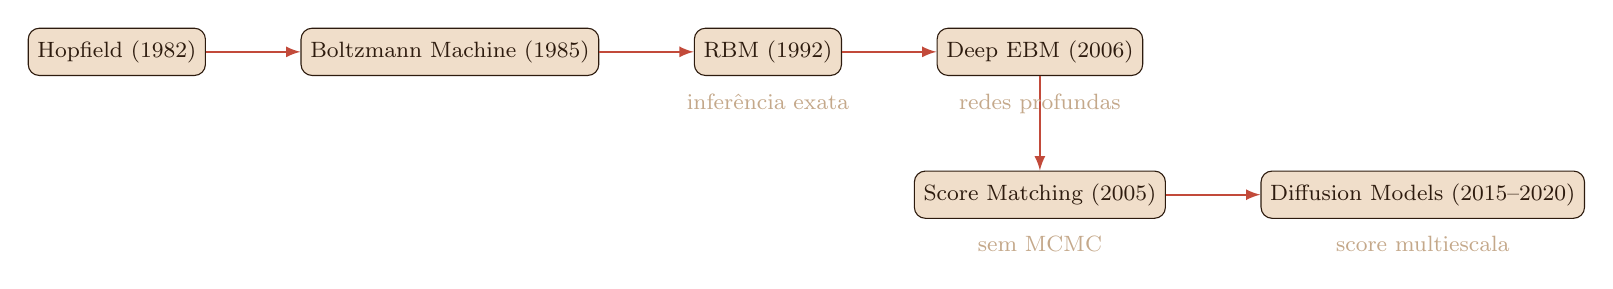
\begin{tikzpicture}[
    node distance=1.2cm,
    auto,
    font=\small,
    >=latex
  ]
  \tikzset{
    nodebox/.style={draw=wp-text, fill=wp-light, rounded corners, minimum width=1.8cm, minimum height=0.6cm, text=wp-text, align=center, font=\footnotesize},
    arrow/.style={->, wp-primary, thick}
  }

  \node (hopfield) [nodebox] {Hopfield (1982)};
  \node (bm) [nodebox, right=of hopfield] {Boltzmann Machine (1985)};
  \node (rbm) [nodebox, right=of bm] {RBM (1992)};
  \node (deep) [nodebox, right=of rbm] {Deep EBM (2006)};
  \node (sm) [nodebox, below=of deep] {Score Matching (2005)};
  \node (diff) [nodebox, right=of sm] {Diffusion Models (2015--2020)};

  \draw[arrow] (hopfield) -- (bm);
  \draw[arrow] (bm) -- (rbm);
  \draw[arrow] (rbm) -- (deep);
  \draw[arrow] (deep) -- (sm);
  \draw[arrow] (sm) -- (diff);

  \node[wp-muted, font=\footnotesize, below=0.1cm of rbm] {inferência exata};
  \node[wp-muted, font=\footnotesize, below=0.1cm of deep] {redes profundas};
  \node[wp-muted, font=\footnotesize, below=0.1cm of sm] {sem MCMC};
  \node[wp-muted, font=\footnotesize, below=0.1cm of diff] {score multiescala};
\end{tikzpicture}
}
\caption{Evolução histórica dos modelos baseados em energia, desde as Redes de Hopfield até os Diffusion Models modernos. Cada passo adiciona uma capacidade fundamental: inferência eficiente (RBM), profundidade (Deep EBM), treinamento sem MCMC (Score Matching), e modelagem multiescala (Diffusion).}
\label{fig:ebm-tree}
\end{figure*}

\subsubsection{Treinamento na Prática: Arquiteturas e Estabilização}

O treinamento de EBMs profundas é notoriamente instável. A fase negativa (erguer picos) e a fase positiva (cavar vales) competem, e a Langevin Dynamics pode não amostrar $p_\theta$ fielmente durante o treinamento. Técnicas práticas incluem:

\begin{itemize}
    \item \textbf{Normalização espectral}: Controla a norma de Lipschitz da função de energia, evitando que a paisagem se torne abrupta e difícil de amostrar.
    \item \textbf{Suavização do gradiente}: Penaliza $\|\nabla_x E_\theta(x)\|$ para evitar picos estreitos que a Langevin não consegue explorar.
    \item \textbf{Buffer de amostras}: Mantém um conjunto de amostras geradas recentemente (replay buffer) para inicializar as cadeias MCMC, reduzindo o custo computacional.
    \item \textbf{Two-stage training}: Pré-treino com score matching ou denoising autoencoder antes de fine-tuning com divergência contrastiva.
\end{itemize}

Arquiteturas comuns incluem redes convolucionais residuais (ResNet-EBM) e Transformers com cabeça de energia linear. EBMs latentes introduzem variáveis ocultas $z$ com energia conjunta $E_\theta(x, z)$, aumentando a capacidade expressiva ao custo de inferência mais complexa.

\subsubsection{Relação com Outros Modelos Generativos}

\begin{itemize}
    \item \textbf{VAEs}: Podem ser vistos como EBMs com energia $E(x) = -\log \int p_\theta(x|z)p(z) \, dz$, mas usando uma distribuição de inferência aproximada $q_\phi(z|x)$ para contornar a intratabilidade. A ELBO é um limite superior na energia.
    \item \textbf{GANs}: O discriminador $D(x)$ pode ser interpretado como uma função de energia: $E(x) = -\log D(x)$. A diferença crucial é que GANs treinam um gerador para produzir amostras (evitando MCMC), enquanto EBMs amostram via Langevin.
    \item \textbf{Diffusion Models}: A conexão mais estreita. Diffusion models aprendem $s_\theta(x_t, t) = -\nabla_{x_t} \log p(x_t) = -\nabla_{x_t} E(x_t, t)$ --- o score em cada nível de ruído. São EBMs com score matching multiescala, onde a energia é $E(x, t) = -\log p(x_t)$.
    \item \textbf{Normalizing Flows}: Flows modelam uma transformação invertível explícita; EBMs modelam a densidade implicitamente através da energia. O trade-off é entre tratabilidade (flows podem calcular $p(x)$ exatamente) e flexibilidade (EBMs não têm restrições arquiteturais).
\end{itemize}

\subsubsection{Vantagens e Desvantagens}

\paragraph{Vantagens}
\begin{itemize}
    \item \textbf{Flexibilidade}: Qualquer função diferenciável $\mathbb{R}^d \rightarrow \mathbb{R}$ pode servir como energia, sem restrições de invertibilidade ou dimensionalidade.
    \item \textbf{Unificação}: VAEs, GANs, RBMs e Diffusion podem ser interpretados como casos particulares de EBMs com diferentes escolhas de energia e treinamento.
    \item \textbf{Detecção de anomalias}: A energia é um detector natural de \textit{out-of-distribution} --- amostras fora da distribuição de treinamento tendem a ter energia alta, sem precisar de um classificador separado.
    \item \textbf{Composição}: Funções de energia podem ser somadas para combinar conhecimentos: $E_{\text{total}}(x) = E_1(x) + E_2(x)$ combina restrições de dois modelos.
\end{itemize}

\paragraph{Desvantagens}
\begin{itemize}
    \item \textbf{Amostragem lenta}: Langevin Dynamics requer centenas a milhares de passos para gerar cada amostra, e cada passo exige uma avaliação da rede.
    \item \textbf{Dificuldade de treinamento}: O equilíbrio entre fase positiva e negativa é frágil, e a aproximação MCMC pode levar a instabilidade ou colapso.
    \item \textbf{Qualidade inferior}: Em altas resoluções, a qualidade das amostras geradas por EBMs puros ainda fica atrás de GANs e Diffusion.
    \item \textbf{Cobertura de modos}: A Langevin Dynamics tende a explorar preferencialmente vales profundos, potencialmente ignorando modos de probabilidade significativa mas separados por barreiras de alta energia.
\end{itemize}

\medskip
\noindent Com os EBMs, completamos nosso panorama dos principais paradigmas generativos. A tabela a seguir sintetiza os compromissos de cada abordagem.

\section{Considerações Finais}

Ao longo deste documento, percorremos a evolução dos modelos generativos profundos para síntese de imagens, desde a separação de conteúdo e estilo com CNNs até os Rectified Flow Models e Modelos Baseados em Energia.

\medskip
\noindent\textbf{Tabela comparativa dos modelos generativos.}
Cada modelo é avaliado em eixos objetivos: capacidade de calcular densidade exata, número de passos para amostragem, estabilidade de treinamento, flexibilidade arquitetural e aplicações típicas.

\medskip
\noindent\textbf{Guia de escolha prática.}

\begin{itemize}
    \item \textbf{Precisa de densidade exata?} $\rightarrow$ Normalizing Flow.
    \item \textbf{Precisa de amostragem em tempo real (1 passo)?} $\rightarrow$ GAN, VAE ou Normalizing Flow.
    \item \textbf{Precisa de máxima qualidade visual?} $\rightarrow$ Diffusion ou Rectified Flow (com 4--50 passos).
    \item \textbf{Precisa de estabilidade de treinamento?} $\rightarrow$ VAE, Diffusion, Normalizing Flow ou Rectified Flow.
    \item \textbf{Precisa de espaço latente interpretável?} $\rightarrow$ VAE ou Normalizing Flow.
    \item \textbf{Precisa de detecção de anomalias sem classificador?} $\rightarrow$ EBM (energia como score OOD).
    \item \textbf{Precisa de máxima flexibilidade arquitetural?} $\rightarrow$ Diffusion, EBM ou GAN (sem restrições de invertibilidade).
\end{itemize}

\medskip
\noindent\textbf{Direções futuras.}
A fronteira atual da modelagem generativa move-se em direção a modelos híbridos e unificados:

\begin{itemize}
    \item \textbf{Modelos híbridos}: VAEs com decoders de difusão (VDM), GANs com regularização baseada em energia (EB-GAN), e fluxos retificados condicionados por modelos de difusão para amostragem adaptativa.
    \item \textbf{Consistency Models} (Song et al., 2023): Amostragem em 1--2 passos para modelos de difusão via mapeamento direto ruído-para-dado.
    \item \textbf{Flow Matching} (Lipman et al., 2023): Generalização dos Rectified Flows que simplifica ainda mais o treinamento, substituindo a ODE por uma perda de regressão direta.
    \item \textbf{EBMs neurais modernas}: Combinando score matching com arquiteturas transformer e técnicas de regularização para superar as limitações de escala dos EBMs clássicos.
    \item \textbf{Modelos unificados}: Frameworks que tratam diferentes paradigmas (difusão, fluxo, energia) como instâncias de uma mesma formulação matemática, permitindo alternar entre eles conforme a necessidade.
\end{itemize}

\end{document}